%This is the presentation template Christine P'ng made (and uses)
%It uses a different theme and different fonts

\documentclass{beamer}
%\documentclass[handout]{beamer}

%\usetheme{Boadilla}

\usepackage[french]{babel}
\usepackage{hyperref}
\usepackage{libertine}
\usepackage[T1]{fontenc}
\usepackage[utf8x]{inputenc}
\usepackage{subfig}
\usepackage{xcolor}
\usepackage{colortbl}
\usepackage{listings}
\usepackage{tikz}
\usepackage{marvosym}
%\usepackage{tikzsymbols}
 \usepackage[marvosym]{tikzsymbols}
\usetikzlibrary{arrows.meta}
\usepackage{environ}
\usepackage{multirow}
\usepackage{multicol}
\usepackage{rotating}
\usepackage[ampersand]{easylist}
\usepackage{wasysym}
\usepackage{booktabs}
\usepackage{centernot}
\usetikzlibrary{shapes,arrows,decorations.pathmorphing,decorations.pathreplacing,backgrounds,positioning,fit,petri}
\usepackage{ulem}
\usepackage{cancel}
\usepackage{tikz}
\usetikzlibrary{arrows}
\usepackage{appendixnumberbeamer}

\definecolor{gcblue}{RGB}{66,126,214} % sampled with Gimp
\definecolor{customRed}{RGB}{240,80,80}
\definecolor{faintred}{RGB}{255,175,175}
\definecolor{faintblue}{RGB}{110,220,255}
\definecolor{faintgray}{RGB}{225,225,225}
\definecolor{titlefontblue}{RGB}{45,45,80}
\definecolor{titlefontcolour}{RGB}{75,75,75}

\usecolortheme[named=titlefontcolour]{structure}
\setbeamersize{text margin left=10mm}
\setbeamertemplate{frametitle}{\vspace{1.5cm}\insertframetitle}
\usefonttheme{serif} %serif

%Setting a different font family for the title and frame titles
%Short titles and headers are required because the font size is set to very large (feel free to change this based on presentation requirements)
% ##### \setbeamerfont{title}{family=\fontfamily{cmr}}
\setbeamerfont{title}{family=\fontfamily{cmss}}
\setbeamerfont{title}{family=\sffamily} %sffamily
\setbeamerfont{title}{size=\fontsize{33}{33}\bfseries}%make this smaller if your title is too long (do the same for the frametitles, etc)
\setbeamerfont{frametitle}{family=\sffamily}
\setbeamerfont{frametitle}{size=\Huge\bfseries}
\setbeamerfont{author}{size=\normalsize\scshape}
\setbeamerfont{institute}{size=\small\scshape}
\setbeamerfont{date}{size=\small\scshape}
\setbeamerfont{subtitle}{size=\small}
\setbeamerfont{normal text}{size=\Huge}

\setbeamertemplate{navigation symbols}{}
\setbeamertemplate{footline}[frame number]{}
\setbeamertemplate{itemize items}[ball]
%\setbeamercolor{itemize items}{fg=blue}
%\setbeamertemplate{itemize item}{\color{yellow}$\blacksquare$}

%\setbeamercolor{itemize item}{fg=red}
%\setbeamercolor{itemize item}{bg=red}

%Adding page numbers at the bottom of each frame
%\setbeamertemplate{footline}
%{%
%  \leavevmode%
%  \hbox{%
%  \begin{beamercolorbox}[wd=1\paperwidth,ht=2.25ex,dp=1ex,right]{date in head/foot}%
%   % \usebeamerfont{date in head/foot}\insertshortdate{}\hspace*{2em}
%    \insertframenumber{} / \inserttotalframenumber\hspace*{2ex} 
%  \end{beamercolorbox}}%
%  \vskip0pt%
%}

%Header Info
% information not capitalized because fonts are set to small caps (looks cleaner this way)
%\title[SRSWOR CLT]{
%	\mbox{} \vskip 2.0cm
%	%{\color{white}Statistics + Algebraic Geometry $=$ $?$}
%	\vskip 0.1cm
%	\small
%	%{\color{white}Identifiability}
%	}


%\author{\vskip -1.5cm\LARGE%\color{titlefontcolour}
%Kenneth Chu}

%\institute[oicr]{\scriptsize
%	\color{titlefontcolour}
%	\inst{}
%	Special Surveys, Transportation, Technology and Quality Assurance, BSMD
%	\vskip 0.0cm
%	Enqu\^{e}tes sp\'{e}ciales, transport, technologie et assurance de la qualit\'{e}, DMEE
%	}

%\date{\color{titlefontcolour}October 21, 2015} 

%%%%%%%%%%%%%%%%%%%%%%%%%%%%%%%%%%%%%%%%%%%%%%%%%%
\begin{document}

\addtocounter{framenumber}{-1}
{
% Titlepage
\usebackgroundtemplate{
\includegraphics[width=\paperwidth,height=\paperheight]{StatCan-presentation-titlePage-background.jpg}}
\begin{frame}[plain]
%\titlepage

\begin{center}

\vskip 2.75cm
\resizebox{0.95\linewidth}{!}{\color{titlefontblue}\bf\itshape Classification}
\resizebox{0.35\linewidth}{!}{\color{titlefontblue}\bf\itshape Trees}

\vskip 0.5cm
\textbf{\large\color{titlefontcolour}Kenneth Chu}

\vskip 0.2cm
\textbf{\scriptsize\color{titlefontcolour}Centre de ressources en analyse de donn\'{e}es, DCIMSI
\vskip -0.1cm
Data Analysis and Resource Centre, ICCSMD}

%\vskip 0.5cm
%\textbf{\large\color{titlefontcolour}Kenneth Chu, Joanne Leung}

%\vskip 0.2cm
%\textbf{\color{titlefontcolour}DMEE / BSMD}

\vskip 0.2cm
\textbf{\color{titlefontcolour}February 23, 2018} 

\end{center}

\end{frame}
}

% Outline
%\begin{frame}{Outline}
%\tableofcontents
%\end{frame}

%%%%%%%%%%%%%%%%%%%%%%%%%%%%%%%%%%%%%%%%%%%%%%%%%%
\newcommand{\graphicsDir}{graphics}
\newcommand*\rot{\rotatebox{90}}
\renewcommand{\Re}{\mathbb{R}}
\newcommand{\N}{\mathbb{N}}
\renewcommand{\d}{\textnormal{d}}
\newcommand{\Var}{\textnormal{Var}}

\definecolor{bgOrange}{RGB}{255,229,204}
\definecolor{lightOrange}{RGB}{220,153,136}

%\definecolor{lightBlue}{RGB}{204,229,225}
\definecolor{lightBlue}{RGB}{0,200,200}

%\definecolor{lessDeepGreen}{RGB}{153,255,204}
\definecolor{lessDeepGreen}{RGB}{0,201,100}

%\definecolor{deepGreen}{RGB}{0,153,76}
\definecolor{deepGreen}{RGB}{0,115,57}

%\definecolor{darkYellow}{RGB}{210,210,0}
\definecolor{darkYellow}{RGB}{200,200,0}

\definecolor{lightTurquoise}{RGB}{153,255,255}
\definecolor{lightYellow}{RGB}{255,255,204}
\definecolor{lightGreen}{RGB}{204,255,204}
\definecolor{darkGreen}{RGB}{128,255,0}
\definecolor{veryDarkGreen}{RGB}{100,225,100}
\definecolor{lightGray}{RGB}{224,224,224}
\definecolor{mediumLightGray}{RGB}{176,176,176}
\definecolor{mediumGray}{RGB}{128,128,128}

\setlength{\arrayrulewidth}{0.55pt}
\arrayrulecolor{mediumGray}

%%%%% ~~~~~~~~~~~~~~~~~~~~ %%%%%
\usebackgroundtemplate{
\includegraphics[width=\paperwidth,height=0.0825\paperwidth]{StatCan-presentation-body-topBanner.jpg}}

%\setlength{\parskip}{0.3cm}


          %%%%% ~~~~~~~~~~~~~~~~~~~~ %%%%%

\section{Overview}
\setcounter{theorem}{0}
\setcounter{equation}{0}

%\cite{vanDerVaart1996}
%\cite{Kosorok2008}

%\renewcommand{\theenumi}{\alph{enumi}}
%\renewcommand{\labelenumi}{\textnormal{(\theenumi)}$\;\;$}
\renewcommand{\theenumi}{\roman{enumi}}
\renewcommand{\labelenumi}{\textnormal{(\theenumi)}$\;\;$}

          %%%%% ~~~~~~~~~~~~~~~~~~~~ %%%%%

\begin{itemize}
\item
	Background (interpretability of linear models):
	
	Linear models have the following form:
	\begin{equation*}
	f(\,x\,;\,\beta\,)
	\;\; = \;\;
		f(\,x_{1},\ldots,x_{p}\,;\,\beta_{0},\beta_{1},\ldots,\beta_{p}\,)
	\;\; = \;\;
		\beta_{0} \,+\, \beta_{1}\cdot x_{1} \,+\, \cdots \,+\, \beta_{p}\cdot x_{p}
	\end{equation*}
	Linear models are deemed ``interpretable'' in at least two ways:
	\begin{enumerate}
	\item
		\label{additiveModelDecomposition}
		The quantity
		\,$\left(\,f(x;\beta) \overset{{\color{white}.}}{-} \beta_{0}\,\right)$\,
		--- the prediction made by the model $f$ on the unlabelled observation $x$
		minus the intercept term $\beta_{0}$ --- is a sum of $p$ summands,
		with each summand $\beta_{i}\cdot x_{i}$ being interpreted as the contribution to 
		\,$\left(\,f(x;\beta) \overset{{\color{white}.}}{-} \beta_{0}\,\right)$\,
		due to the $i^{\textnormal{th}}$ predictor variable, for $i = 1,\ldots,p$.
	\item
		\label{beteInterpretability}
		$\beta_{0} = f(\,0,\ldots,0\,;\,\beta\,)$ is the prediction by $f$ on $x = (0,\ldots,0)$,
		while each $\beta_{i}$ can be interpreted as the change in $f(\,x\,;\,\beta\,)$
		caused by each unit change in $x_{i}$, for $i = 1,\ldots,p$.
	\end{enumerate}
\item
	What about nonlinear models?
	
	For a model $f(\,x\,;\,\beta\,)$ nonlinear in $\beta$, interpretability in the sense of
	\eqref{beteInterpretability} above is obviously highly nontrivial, if not impossible.
	But, it begs the question:
	\begin{center}
	\vskip -0.2cm
	\textbf{\color{red}Even for nonlinear models, can \eqref{additiveModelDecomposition}
	be achieved in some (satisfying/useful) sense?}
	\end{center}

\item
	An example of using the Shapley decomposition to achieve \eqref{additiveModelDecomposition}
	for arbitrary models (including nonlinear models):
	
	\v{S}trumbelj-Kononenko \cite{Strumbelj2010}
	introduced a method to {\color{red}explain individual predictions}:
	\begin{itemize}
	\item
		Given a trained prediction model $f(X_{1},\ldots,X_{p})$
		based on a set of predictor variables $(X_{1},\ldots,X_{p})$, and
		an unlabelled observation $x = (x_{1},\ldots,x_{p})$,
		\v{S}trumbelj-Kononenko \cite{Strumbelj2010} shows that
		one can assign a ``contribution score'' $R_{i}(x;f)$
		to each predictor variable $X_{i}$
		such that the following equality holds:
		\begin{equation*}
		f(x) \, - \, A_{0}(f)
		\;\; = \;\;
			\overset{p}{\underset{i=1}{\sum}}\;
			R_{i}(x;f)\,,
		\end{equation*}
		where $A_{0}(f)$ is the average of the predictions by $f$
		over all possible combinations of predictor values.

		\vskip 0.2cm
		\textbf{Thus, the contribution score $R_{i}(x;f)$ can be interpreted
		as the ``{\color{red}contribution}'' to the quantity \,$\left(\,f(x) - A_{0}(f)\,\right)$\,
		 --- the prediction made by $f$ on $x$ minus the average prediction of $f$ ---
		due to the $i^{\textnormal{th}}$ predictor value $X_{i} = x_{i}$,
		in relation to all the other predictor values
		$X_{1} = x_{1}$, \,$\ldots$\;, $X_{p} = x_{p}$.}
		\vskip 0.2cm
		
	\item
		The $i^{\textnormal{th}}$ contribution score $R_{i}(x;f)$ above
		turns out to be the $i^{\textnormal{th}}$ {\color{red}Shapley value} of
		a certain {\color{red}Shapley decomposition}.
		See Definition \eqref{definition:ShapleyDecomposition}.
	\end{itemize}

\item
	The Shapley decomposition is a notion
	in game theory\footnote{more precisely, cooperative game theory, a.k.a. coalitional game theory}
	first introduced in \cite{Shapley1953}.
	Its underlying intuitive idea is as follows:

	Suppose:
	\begin{itemize}
	\item
		$U$ is a finite population of ``players''.
	\item
		A \textit{coalition} is a subset of players from $U$.
		(Think: a coalition is just a team of players chosen from $U$.)
	\item
		There is a (coalition-level) \textit{score} assigned to every possible coalition
		and the score of the ``empty coalition'' (the coalition with zero players) is zero.
	\end{itemize}
	
	The objective of the Shapley decomposition is to ``distribute'' the population score
	(the coalition-level score for the whole population of players)
	to each of the individual players such that
	\begin{itemize}
	\item
		the individual scores always simply just {\color{red}add back up} to the population score, and
	\item
		all the (possibly extremely complicated) {\color{red}interactions}
		among the players are taken into account.
	\end{itemize}
	
	Shapley proves in \cite{Shapley1953} the following (rather remarkable) result:
	If we insist that the Shapley decomposition should possess
	certain ``natural/desirable'' properties
	(see Definition \ref{definition:ShapleyDecomposition}),
	then, given any coalition-level score, its Shapley decomposition exists and is unique
	(or, intuitively speaking, there is {\color{red}one and only one} way to distribute
	the population score to the individual players in a ``natural'' manner).
	See Theorem \ref{theorem:ShapleyDecompositionExistenceUniqueness}
	(for the existence, uniqueness, and explicit formula of the Shapley decomposition).

	The explicit formula in
	Theorem \ref{theorem:ShapleyDecompositionExistenceUniqueness}
	shows that the Shapley decomposition takes into account
	the interactions among all players by,
	for each given player, {\color{red}suitably averaging} his/her {\color{red}marginal scores}
	over all possible coalitions containing that given player
	(in other words, the Shapley decomposition does this by very clever bookkeeping).

\item
	We now give an outline of \v{S}trumbelj-Kononenko \cite{Strumbelj2010}:

	\begin{itemize}
	\item
		\v{S}trumbelj-Kononenko \cite{Strumbelj2010} applies
		the Shapley decomposition %to these choices of $U$ and $\nu(S;x,f)$ 
		to define their contribution scores $R_{i}(x,f)$.
		
		More precisely, \v{S}trumbelj-Kononenko \cite{Strumbelj2010}
		chooses the population $U$ of players to be the set of features (predictor variables),
		i.e. $U = \{X_{1},\ldots,X_{p}\}$.
		A coalition is thus a (sub-)selection $S$ of features from $U$.
		By Theorem \ref{theorem:ShapleyDecompositionExistenceUniqueness},
		the Shapley decomposition $\varphi$ on $U$ exists and is unique.

		It now remains only to choose a suitable coalition-level score $\nu(S;x,f)$.
		Once that choice is made, we can define the $i^{\textnormal{th}}$ contribution score
		$R_{i}(x;f)$ simply to be the $i^{\textnormal{th}}$ Shapely value of
		$\varphi\left(\,\nu(\,\cdot\,;\,x,f)\,\right)$.

	\item
		Choice of coalition-level score $\nu(S;x,f)$:
		
		In \cite{Strumbelj2010},
		each feature is assumed to be a categorical variable
		with finitely many levels;
		in particular, the entire feature space is finite.

		
		The coalition-level score $\nu(S;x,f)$ is chosen to be the difference
		$A(S;x,f) - A_{0}(f)$
		of two averages of predictions, where $A_{0}(f)$ is as before
		the average of the predictions by $f$ over all possible combinations of feature values,
		while $A(S;x,f)$ is the average of the predictions by $f$ over only those combinations
		$(z_{1},\ldots,z_{p})$ such that $z_{i} = x_{i}$ for each $i \in S$.
		%\v{S}trumbelj-Kononenko \cite{Strumbelj2010} applies
		%the Shapley decomposition to these choices of $U$ and $\nu(S;x,f)$ 
		%in order to obtain their contribution scores $R_{i}(x,f)$.
		%See \cite{Strumbelj2010} for precise mathematical formulation.

	\item
		For completeness, we show the definition of $\nu(S;f,x)$ here:
		\begin{equation*}
		\nu(S;f,x)
		\;\; := \;\;
			\dfrac{1}{{\color{white}.}\vert\,\mathcal{F_{\,U\,\backslash S}}\,\vert{\color{white}.}}
			\cdot
			\underset{\xi\,\in\,\mathcal{F}_{U \backslash S}}{\sum}f(\tau(x,\xi;S))
			\; - \;
			\dfrac{1}{{\color{white}.}\vert\,\mathcal{F}\,\vert{\color{white}.}}
			\cdot
			\underset{\xi \in \mathcal{F}}{\sum}\;f(y)
		\end{equation*}
		where $\mathcal{F}$ is the feature space, and
		\begin{equation*}
		\tau(x,\xi;S) \;\; = \;\; (z_{1},\ldots,z_{p})\,,
		\quad\quad
		z_{i}
		\; = \;
			\left\{\begin{array}{cl}
			x_{i}, & i \in S
			\\
			\xi_{i}, & i \notin S
			\end{array}\right.
		\end{equation*}
		However, we omit the definition of $\mathcal{F}_{U\,\backslash S}$ above and
		refer the reader to \cite{Strumbelj2010} for full mathematical details.

	\item
		The explicit formula in
		Theorem \ref{theorem:ShapleyDecompositionExistenceUniqueness}
		shows that a straightforward implementation of the Shapley decomposition
		has exponential computational complexity.
		One of the main contributions in \cite{Strumbelj2010} is
		an effective and efficient procedure to approximate
		the Shapley decomposition in the given context.

	\item
		The {\color{red}R package} 
		\texttt{iml} \cite{Molnar2018} %(\texttt{https://CRAN.R-project.org/package=iml})
		provides implementations for a number of interpretability methods,
		including that of \v{S}trumbelj-Kononenko \cite{Strumbelj2010}.

	\end{itemize}

\item
	There are, of course, variations to the interpretability method described in \cite{Strumbelj2010};
	see for example, \cite{Lipovestsky2001} and \cite{Lundberg2017}. 

\item
	For a more comprehensive discussion on interpretable machine learning
	(including approaches other than those based on the Shapley decomposition),
	see the {\color{red}online book} \cite{Molnar2019}.

\end{itemize}

          %%%%% ~~~~~~~~~~~~~~~~~~~~ %%%%%

%\renewcommand{\theenumi}{\alph{enumi}}
%\renewcommand{\labelenumi}{\textnormal{(\theenumi)}$\;\;$}
\renewcommand{\theenumi}{\roman{enumi}}
\renewcommand{\labelenumi}{\textnormal{(\theenumi)}$\;\;$}

          %%%%% ~~~~~~~~~~~~~~~~~~~~ %%%%%



%%%%%%%%%%

\begin{frame}{\Large \vskip -0.5cm L'ensemble de donn\'ees Iris de R.A. Fisher\\ \small(3 esp\`eces, 50 observations chacune)
\vskip -0.1cm{\tiny Fisher, R.A. \textit{The use of multiple measurements in taxonomic problems}, Annual Eugenics, 7, Part II, 179-188 (1936)}
}

\small

\begin{multicols}{2}

	\begin{flushleft}
	%\mbox{} \vskip -0.75cm
	\begin{minipage}{4.5cm}
	\vskip -0.2cm
	\begin{center}
	$\textnormal{Iris setosa}$
	\vskip 0.05cm
	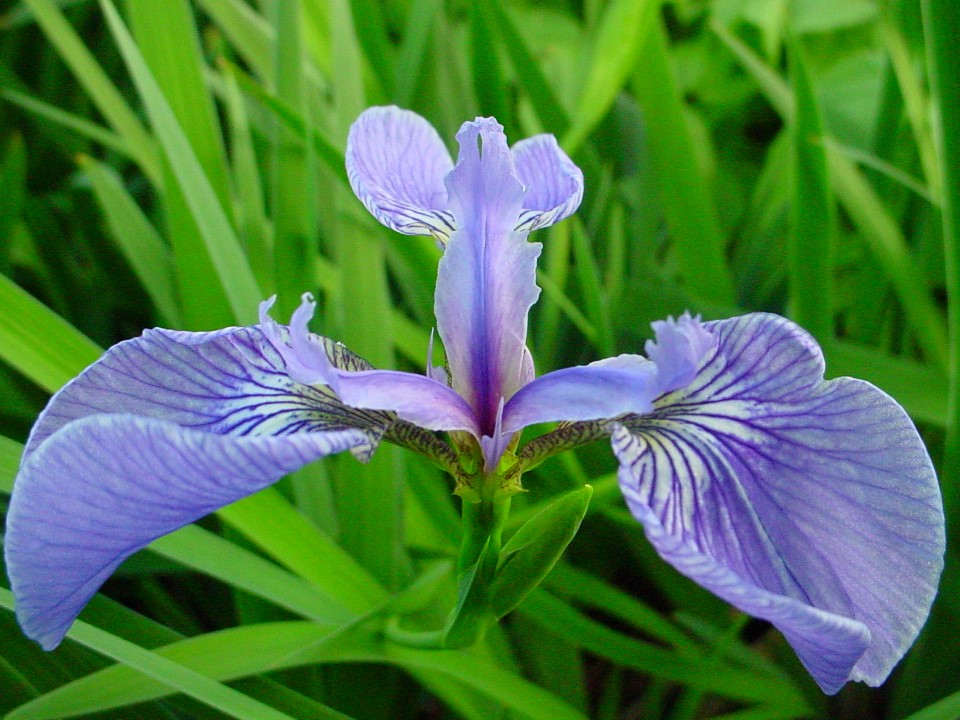
\includegraphics[width=3.5cm]{graphics/Iris-setosa-var-canadensis.png}
	\end{center}
	\end{minipage}
	\end{flushleft}

\columnbreak

	\begin{flushright}
	\begin{minipage}{4.5cm}
	\vskip -0.2cm
	\begin{center}
	$\textnormal{Iris versicolor}$
	\vskip 0.05cm
	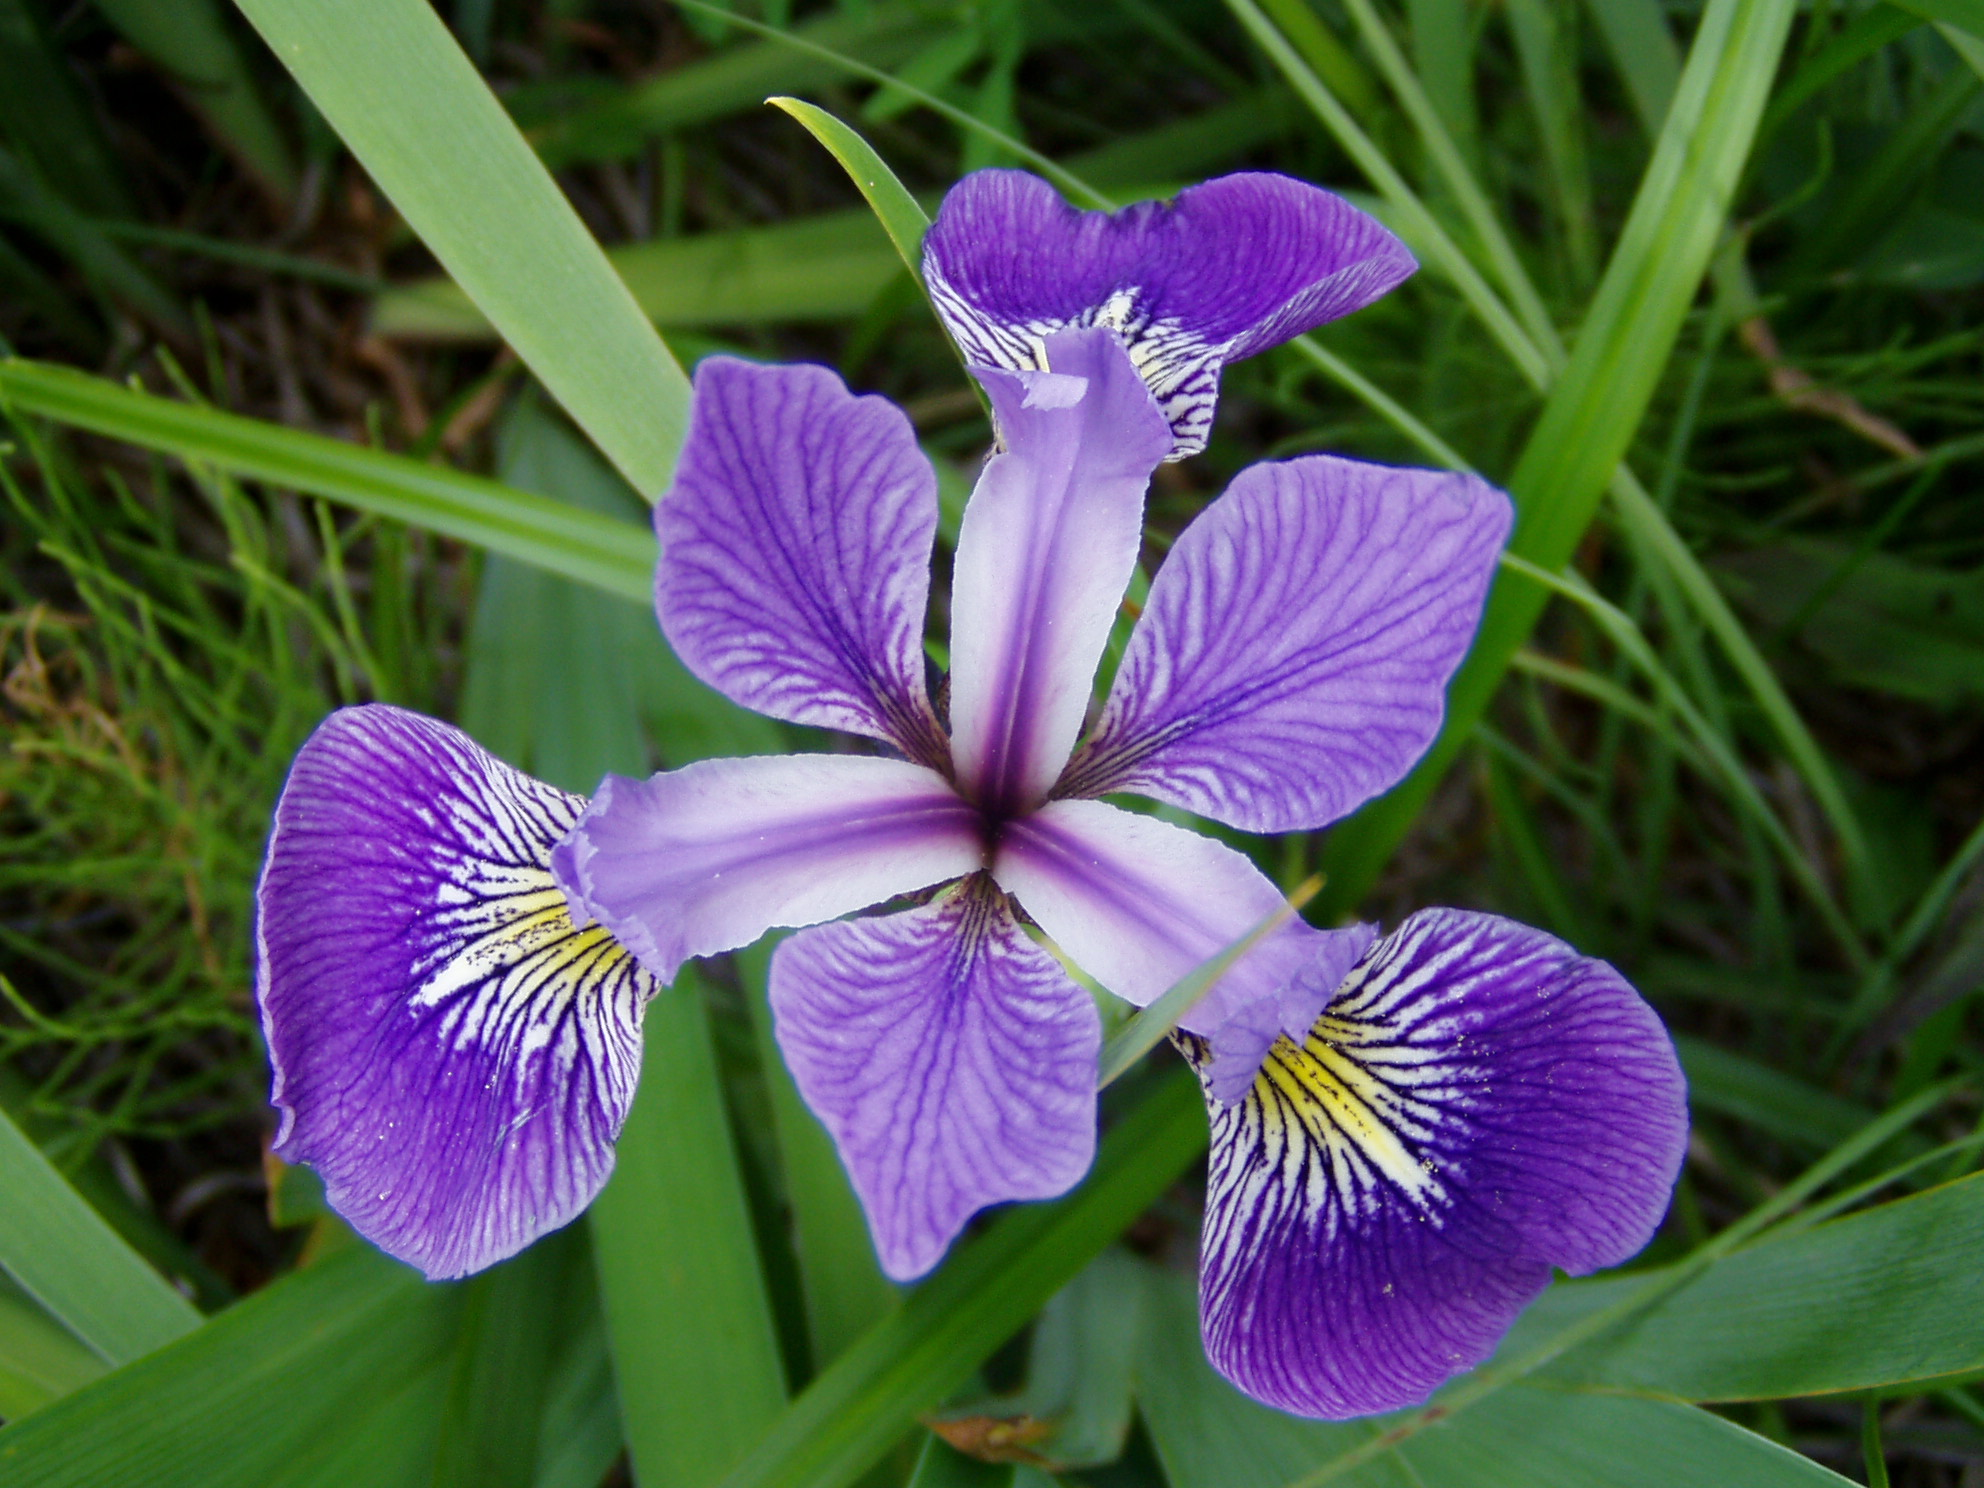
\includegraphics[width=3.5cm]{graphics/Iris-versicolor-3.png}
	\end{center}
	\end{minipage}
	\end{flushright}

\end{multicols}

\begin{multicols}{2}

	\begin{flushleft}
	\begin{minipage}{4.5cm}
	%\vskip -0.2cm
	\begin{center}
	$\textnormal{Iris virginica}$
	\vskip 0.05cm
	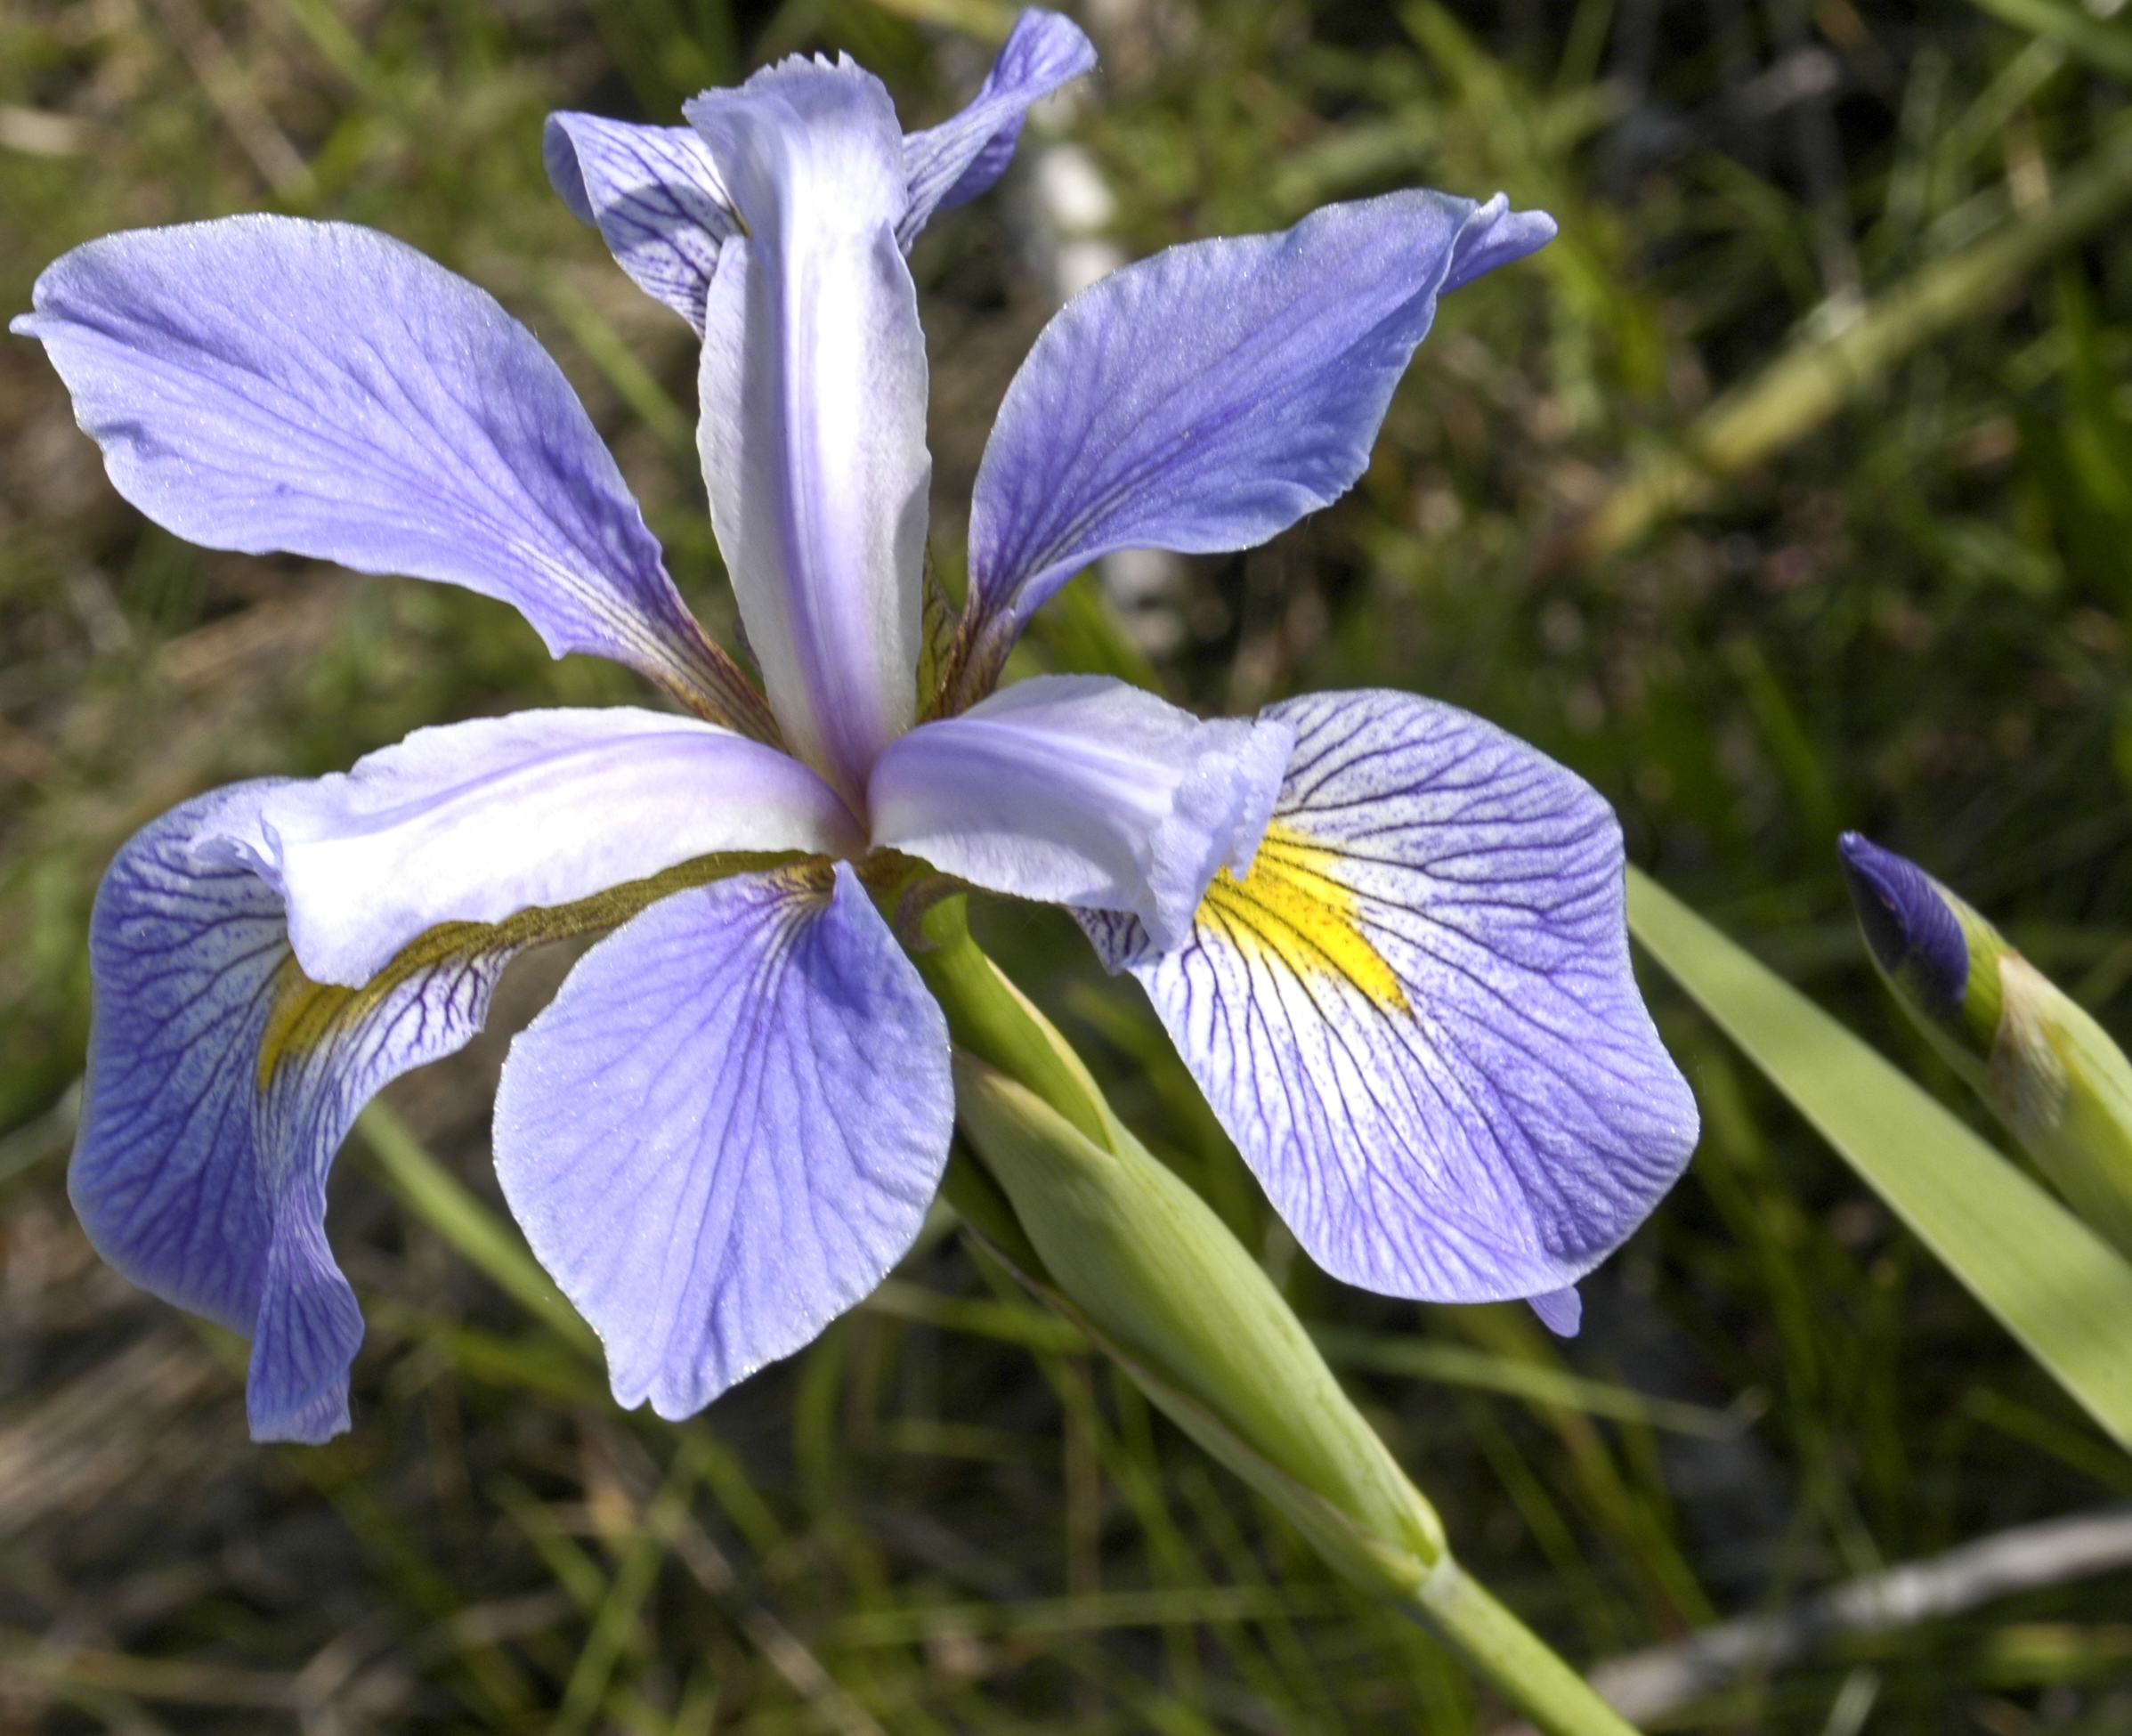
\includegraphics[width=3.5cm]{graphics/Iris-virginica.png}
	\end{center}
	\end{minipage}
	\end{flushleft}

\columnbreak

	\begin{flushright}
	\begin{minipage}{4.5cm}
	%\vskip -0.2cm
	\begin{center}
	\includegraphics[width=3.0cm]{graphics/iris-petal-sepal-278x300.png}
	\end{center}
	\end{minipage}
	\end{flushright}

\end{multicols}

\end{frame}
\normalsize

%%%%%%%%%%

\begin{frame}{\large Entra\^iner un arbre de classification avec \texttt{\normalsize rpart(\,)} de R}

\small

\begin{multicols}{2}

	\begin{flushleft}
	\begin{minipage}{4.5cm}
	\only<1-2|handout:0>{\includegraphics[width=4.5cm]{graphics/scatter-petalLength-vs-petalWidth.png}}
	\only<3-3>{\includegraphics[width=4.5cm]{graphics/scatter-petalLength-vs-petalWidth-boundaries.png}}
	\end{minipage}
	\end{flushleft}

\columnbreak

	\begin{flushright}
	\begin{minipage}{4.5cm}
	\vskip -0.55cm
	\only<1-1|handout:0>{\includegraphics[width=4.5cm,height=6.75cm]{graphics/transparent.png}}
	\only<2-3>{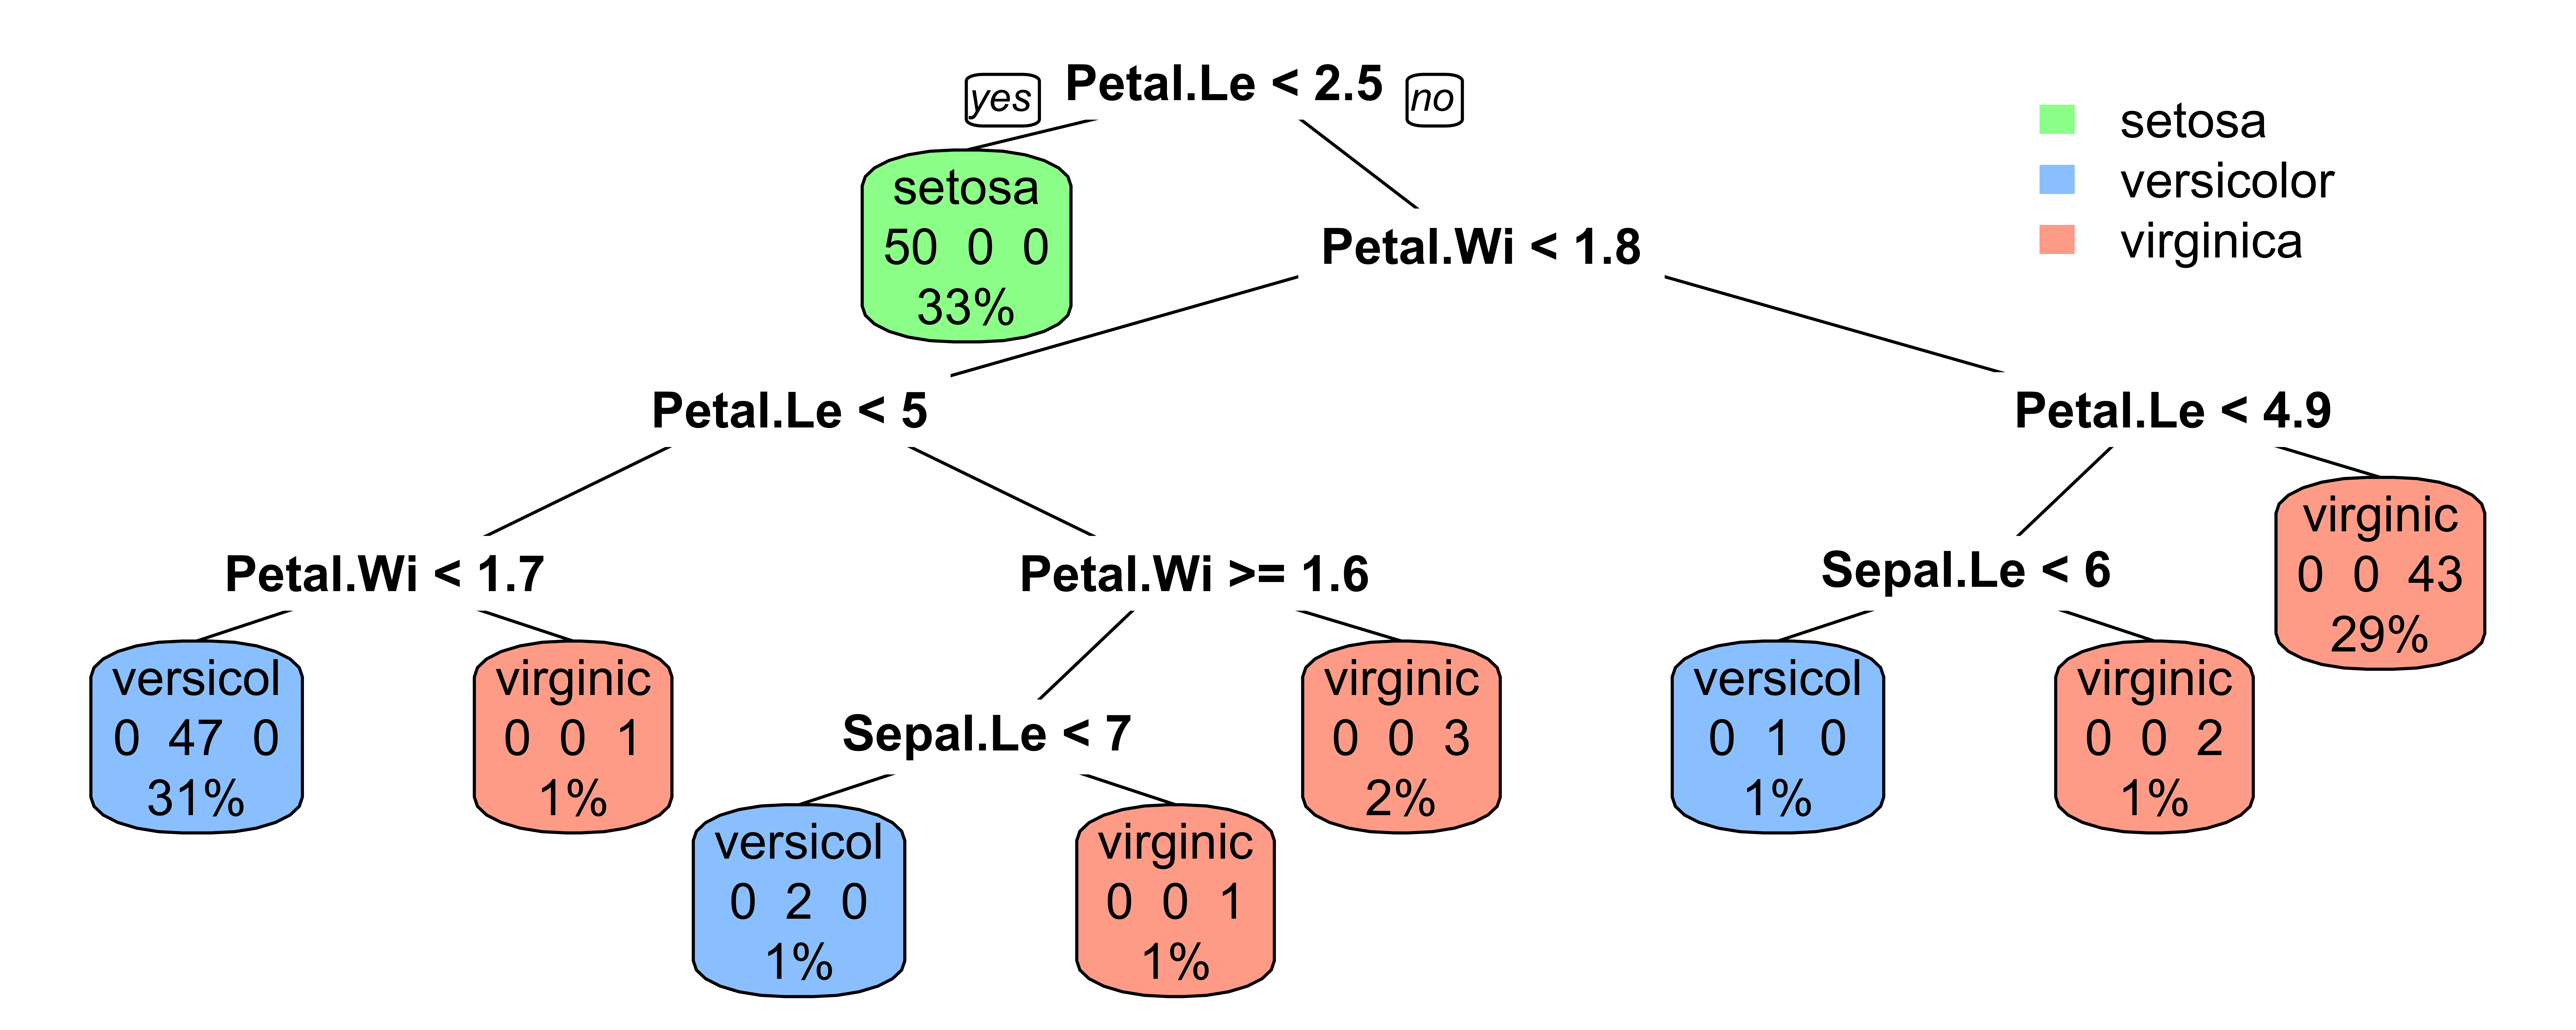
\includegraphics[width=4.5cm,height=6.75cm]{graphics/plot-rpart.png}}
	\end{minipage}
	\end{flushright}

\end{multicols}

\end{frame}
\normalsize

%%%%%%%%%%

%\begin{frame}{\vskip -0.4cm \small Piecewise constant functions generated by\\ \textbf{\Large recursive binary partitioning}}
\begin{frame}{\vskip -0.4cm \small Fonctions constantes par morceau produites par\\ \textbf{\Large partitionnement binaire r\'ecursif}}

\small

\begin{multicols}{2}

	\begin{flushleft}
	\begin{minipage}{4.5cm}
	\includegraphics[width=4.5cm]{graphics/scatter-petalLength-vs-petalWidth-boundaries.png}
	\end{minipage}
	\end{flushleft}

\columnbreak

	\begin{flushleft}
	\begin{minipage}{4.5cm}
	\vskip -0.55cm
	\includegraphics[width=5.5cm,height=6.75cm]{graphics/plot-regression-surface.png}
	\end{minipage}
	\end{flushleft}

\end{multicols}

\end{frame}
\normalsize

%%%%%%%%%%


%%%%%%%%%%

\begin{frame}{\vskip -0.2cm \large The optimization problem behind classification trees}

%\Large
%\begin{center}
%\pause
%Minimize objective function ({\small a.k.a.} cost function)
%\end{center}

\large
\begin{itemize}
\item
	\pause
	Domain ({\small a.k.a.} \,hypothesis class\, {\small a.k.a.} model space)
	\vskip -0.1cm
	{\scriptsize\begin{equation*}
	\pause
	\left\{\begin{array}{c}
		\overset{{\color{white}.}}{\textnormal{recursive}} \\
		\textnormal{binary trees}
	\end{array}\right\}
	\pause
	\quad\sim\quad
	\left\{\begin{array}{c}
		\overset{{\color{white}.}}{\textnormal{piecewise constant functions}} \\
		\textnormal{resulting from} \\
		\textnormal{recursive binary partitioning}
	\end{array}\right\}
	\end{equation*}}

\item
	\pause
	Minimize the objective function ({\small a.k.a} cost function)
	\pause
	\vskip -0.1cm
	{\small\begin{equation*}
	\textnormal{tree impurity}
	\;=\;
		\textnormal{weighted average of leaf impurities}
	\end{equation*}}

\item
	\pause
	\vskip -0.2cm
	The Breiman-Friedman-Olshen-Stone CART
	Algorithm\!\!\footnote{\tiny Breiman-Friedman-Olshen-Stone (1984),
	\textit{{\color{red}C}lassification {\color{red}a}nd {\color{red}R}egression {\color{red}T}rees},
	Taylor \& Francis}
	\begin{itemize}
	\setlength{\itemindent}{-0.175in}
	\item
		\pause
		{\footnotesize Growing: at each step, select ``best'' way to split leaves to get the next tree.}
	\item
		\pause
		{\footnotesize Pruning: prune back fully grown tree to mitigate for overfitting}
	\end{itemize}
\end{itemize}

\end{frame}
\normalsize

%%%%%%%%%%


%%%%%%%%%%

%\begin{frame}{\vskip -0.2cm \large The optimization problem behind classification trees}
\begin{frame}{\vskip -0.4cm \large Le probl\`eme d'optimisation derri\`ere les arbres de classification}

\large
\begin{itemize}
\item
	{\Large Domaine de la fonction objective} {\scriptsize(c.-\`a-d. classe d'hypoth\`eses)}
	{\scriptsize\begin{equation*}
	\left\{\begin{array}{c}
		\overset{{\color{white}.}}{\textnormal{arbres binaires}} \\
		\textnormal{r\'ecursifs}
	\end{array}\right\}
	\quad\sim\quad
	\left\{\begin{array}{c}
		\overset{{\color{white}.}}{\textnormal{fonctions constantes par morceaux}} \\
		\textnormal{resultantes de} \\
		\textnormal{partitionnement binaire r\'ecursif}
	\end{array}\right\}
	\end{equation*}}

	\begin{center}
	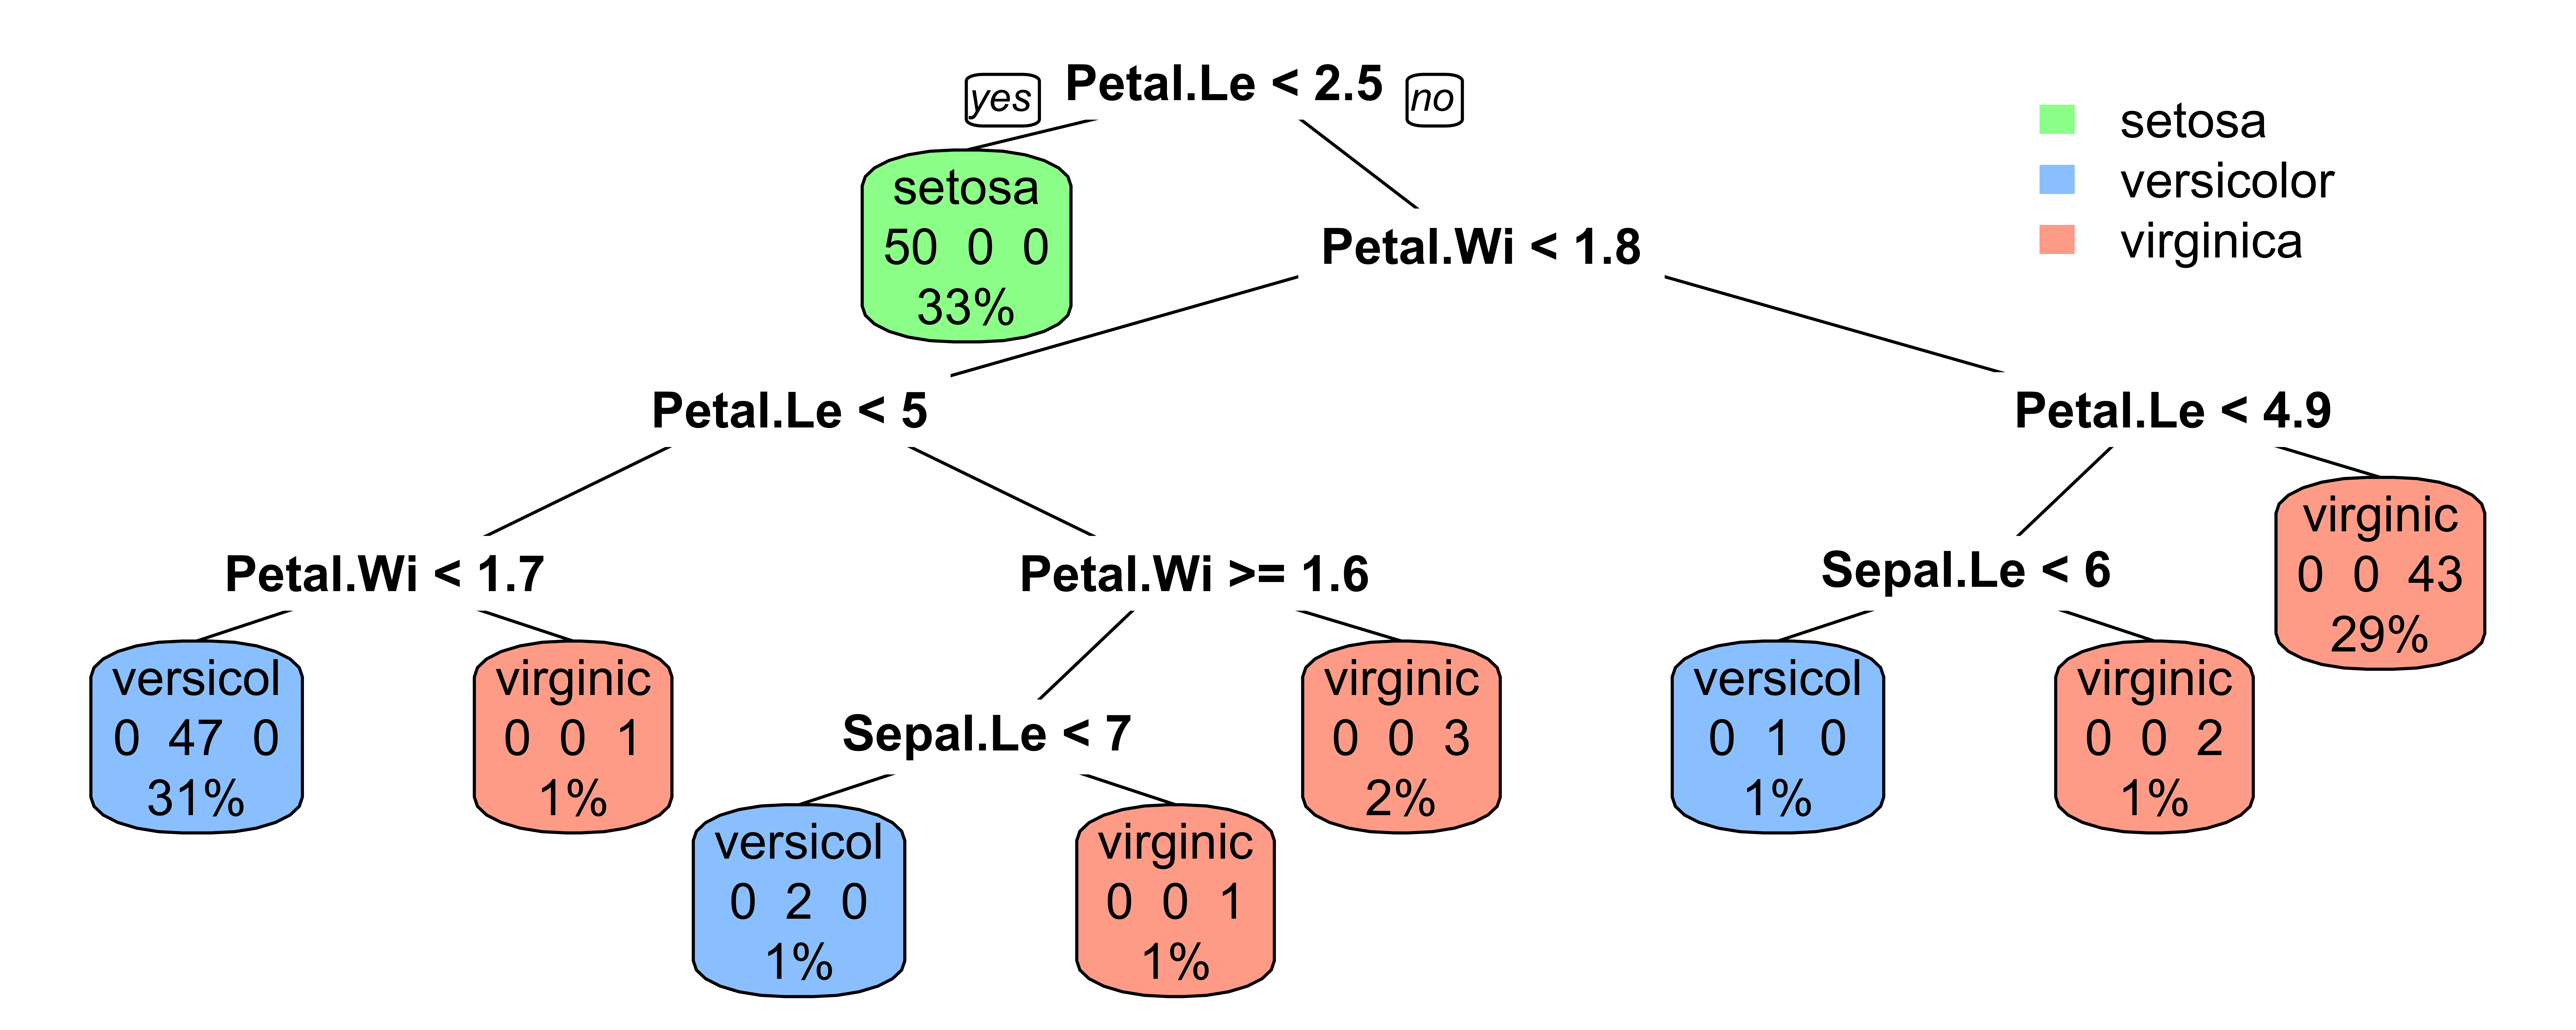
\includegraphics[width=2.5cm,height=3.5cm]{graphics/plot-rpart.png}
	\quad\quad\quad\quad\;\;
	\includegraphics[width=2.5cm,height=3.25cm]{graphics/plot-regression-surface.png}
	\;\;{\color{white}1}
	\end{center}
\end{itemize}


\end{frame}
\normalsize

%%%%%%%%%%


%%%%%%%%%%

\begin{frame}{\vskip -0.45cm \large Le probl\`eme d'optimisation derri\`ere les arbres de classification}

\small

\begin{multicols}{2}

	\begin{flushleft}
	\begin{minipage}{4.5cm}
	\vskip -0.5cm
	
%%%%%%%%%%

%\begin{figure}[h]

\centering
\begin{tikzpicture}

\node at (0,0) {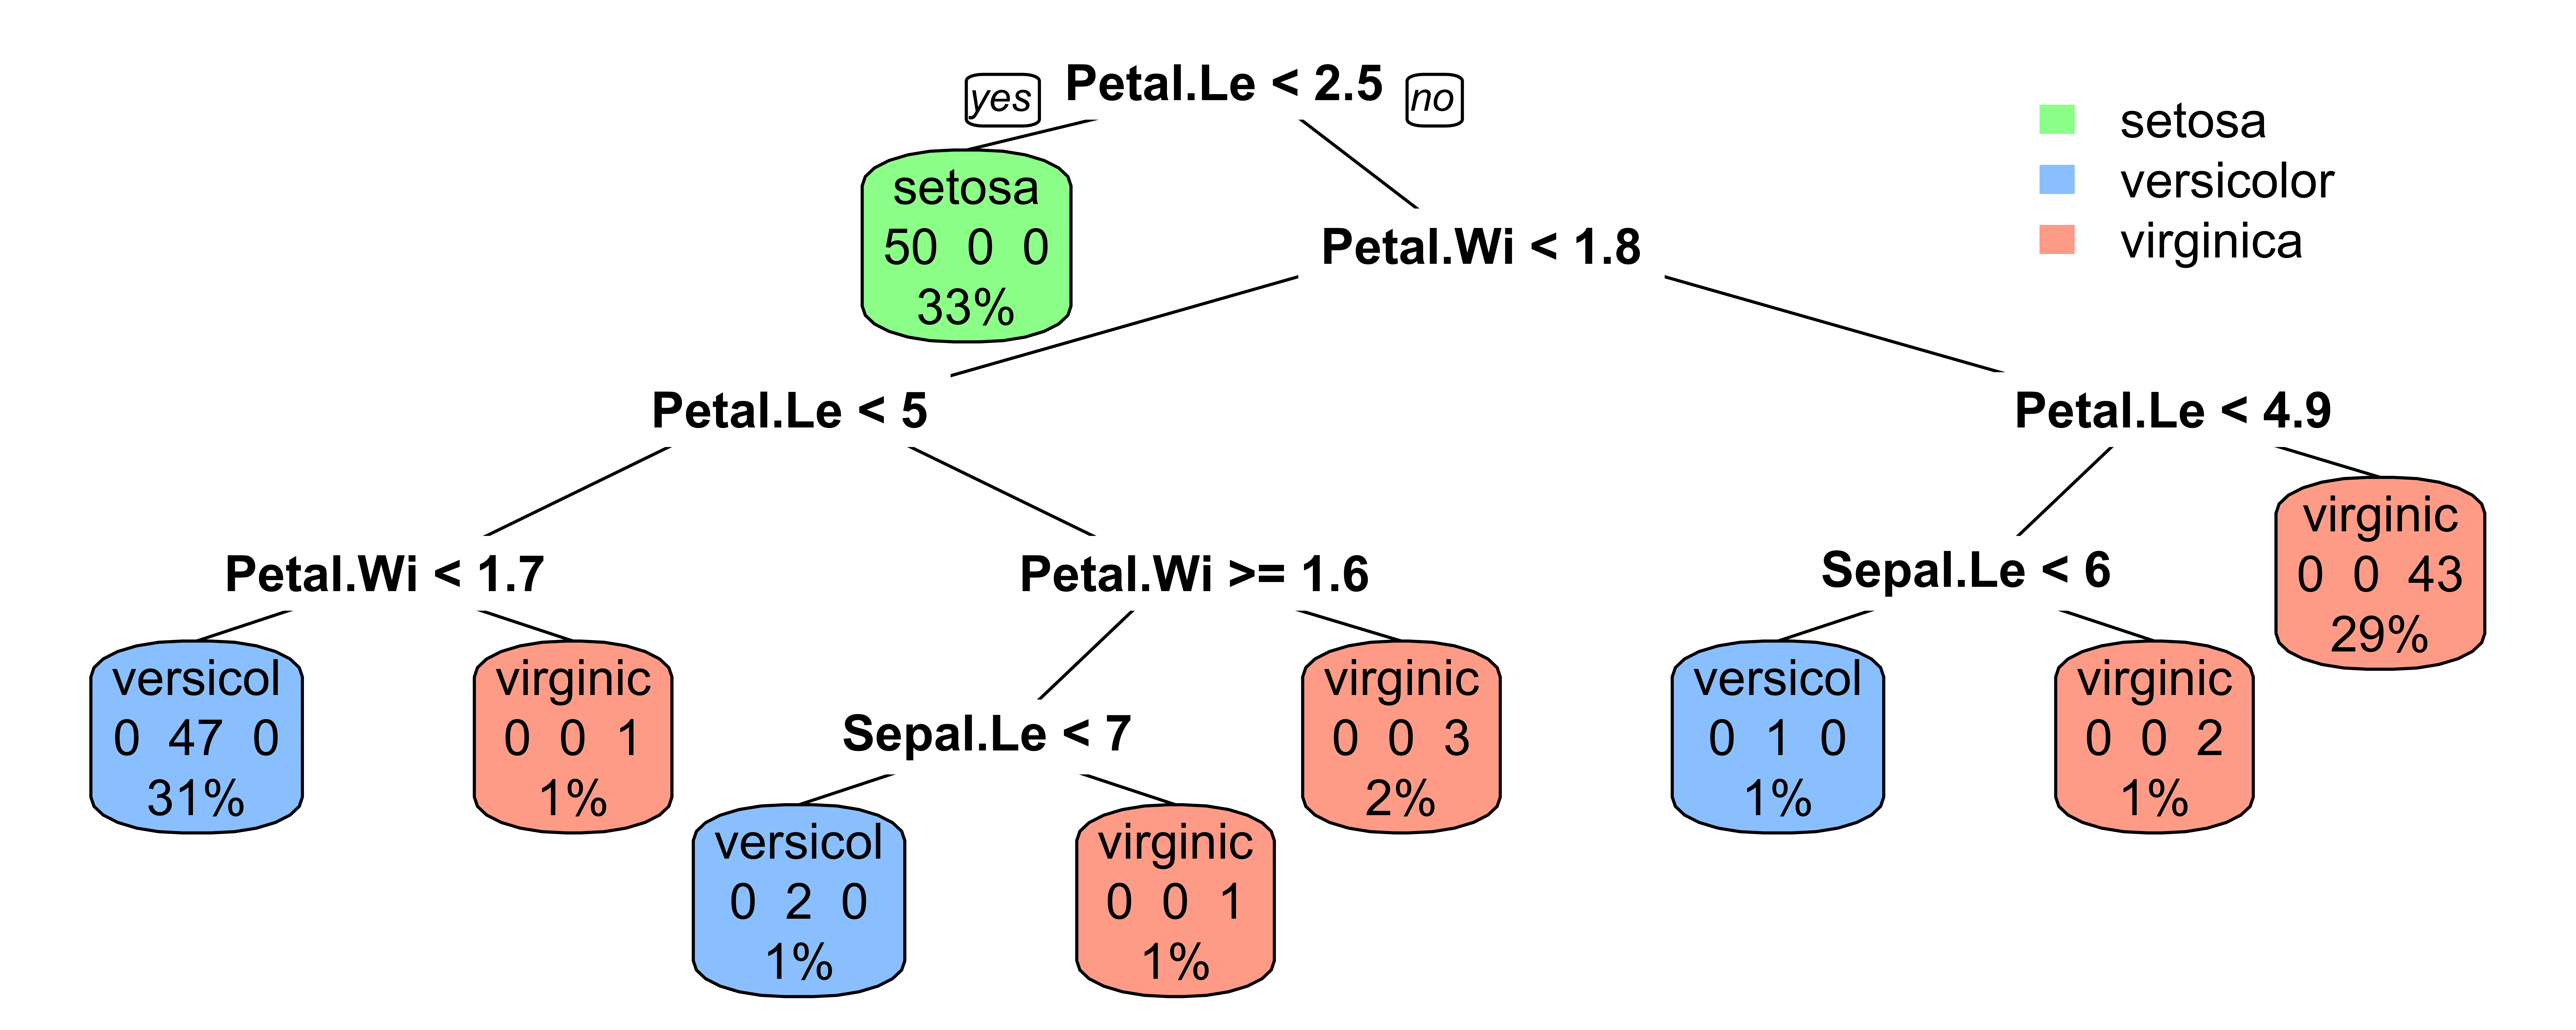
\includegraphics[width=4.5cm,height=6.25cm]{graphics/plot-rpart.png}};

%\node at (-1.55,-0.6) {\scriptsize$H(l_{1}\vert D) = 0$};
%\node at (-0.45,-3.125) {\scriptsize$H(l_{2}\vert D) = 0.445$};
%\node at (1.85,-3.125) {\scriptsize$H(l_{3}\vert D) = 0.151$};

%\node at (-1.55,-0.6) {\scriptsize$G(l_{1}\vert D) = 0$};
%\node at (-0.45,-3.125) {\scriptsize$G(l_{2}\vert D) \approx 0.168$};
%\node at (1.85,-3.125) {\scriptsize$G(l_{3}\vert D) \approx 0.043$};

\node at (-1.55,-0.675) {\scriptsize$G(l_{1}\vert D) = 0$};
\node at (-0.45,-3.15) {\scriptsize$G(l_{2}\vert D) \approx 0.168$};
\node at (1.85,-3.15) {\scriptsize$G(l_{3}\vert D) \approx 0.043$};

%%%  ~~~~~~~~~~  %%%

%%%%%%%%

\end{tikzpicture}

%%%%%%%%%%

	\end{minipage}
	\only<1-7|handout:0>{
		{\color{white}\scriptsize\begin{equation*}
		I(T \vert D) = \frac{50}{150}\times 0 + \frac{54}{150}\times 0.168 + \frac{46}{150} \times 0.043
		\end{equation*}}
		}
	\vskip -0.15cm
	\only<8->{
		{\scriptsize\begin{equation*}
		I(T \vert D) = \frac{{\color{red}50}}{150}\times 0 + \frac{{\color{red}54}}{150}\times 0.168 + \frac{{\color{red}46}}{150} \times 0.043
		\end{equation*}}
		}
	\end{flushleft}

\columnbreak

	\begin{flushright}
	\begin{minipage}{6.0cm}
	\vskip -0.6cm
	\pause
		{\Large Fonction objective}
	\pause
		\begin{center}\textbf{Impuret\'e d'arbres\\ d'apr\`es les donn\'ees}\end{center}
	\pause
		\begin{equation*}
		I(T\,\vert D)
		\; =
			\underset{l\,\in\,\textnormal{Feuilles}(T)}{\sum}\!\!
			P(X \!\in\! l\,) \cdot I(l\,\vert D)
		\end{equation*}
		{\scriptsize o\`u}
		{\scriptsize\begin{eqnarray*}
		\only<1-6|handout:0>{\color{white}
			P(X \!\in\! l\,) &\color{white}=& \color{white}\left(\!\!\!\begin{array}{c}
			\textnormal{probabilit\'e pour}
			\\
			\textnormal{une unit\'e tir\'ee au hasard}
			\\
			\textnormal{de parvenir la feuille $l$}
			\end{array}\!\!\!\!\right)
			}
		\only<7->{
			P(X \!\in\! l\,) &=& \left(\!\!\!\begin{array}{c}
			\textnormal{probabilit\'e pour}
			\\
			\textnormal{une unit\'e tir\'ee au hasard}
			\\
			\textnormal{de parvenir la feuille $l$}
			\end{array}\!\!\!\!\right)
			}
		\only<1-4|handout:0>{
		\\
			\color{white}I(l\,\vert D) &\color{white}=& \color{white}\left(\!\!\begin{array}{c}
				\textnormal{impurity of leaf $l$}
				\\
				\textnormal{given data $D$}
				\end{array}\!\!\right)
			}
		\only<5->{
		\\
			I(l\,\vert D) &=& \left(\!\!\begin{array}{c}
				\textnormal{impuret\'e de la feuille $l$}
				\\
				\textnormal{d'apr\`es les donn\'ees $D$}
				\end{array}\!\!\right)
			}
		\end{eqnarray*}}
	\pause
		\only<1-5|handout:0>{\color{white}\begin{center}
		\vskip -0.5cm
		{\scriptsize Choix communs pour $I(l\,\vert D)$:}
		\vskip 0.1cm
		Entropy ($H$),\;
		Gini Impurity ($G$)
		\end{center}}
		\only<6->{\begin{center}
		\vskip -0.5cm
		{\scriptsize Choix communs pour $I(l\,\vert D)$:}
		\vskip 0.1cm
		Entropie ($H$),\;
		Impuret\'e de Gini ($G$)
		\end{center}}
	\end{minipage}
	\end{flushright}

\end{multicols}

\end{frame}
\normalsize

%%%%%%%%%%

\begin{frame}{\vskip -0.2cm \Large Mesures d'impuret\'e : Entropie \& Impuret\'e Gini}

\vskip -0.2cm
\tiny
\begin{equation*}
I(l\,\vert D)
\;\; = \;\;
\left\{\begin{array}{ccl}
\textnormal{Entropie}
& := &
	\textnormal{\tiny$-\;\overset{C}{\underset{y=1}{\sum}}\;\,
	\widehat{p}(Y=c\,\vert X\in l\,) \cdot \log\,\widehat{p}(Y=c\,\vert X\in l\,)$}
\\
\textnormal{Impuret\'e de Gini}
& := &
	\textnormal{\tiny$+\;\overset{C}{\underset{y=1}{\sum}}\;\,
	\widehat{p}(Y=c\,\vert X\in l\,) \cdot
	\left(\overset{{\color{white}.}}{1}\,-\,\widehat{p}(Y=c\,\vert X\in l\,)\right)$}
\end{array}\right.
\end{equation*}

\begin{multicols}{2}

	\begin{minipage}{4.5cm}
	\begin{flushleft}
	\vskip 0.25cm
	{\scriptsize
	\begin{eqnarray*}
	\pause
	&&
		\textnormal{\normalsize$G\!\left(\left(\frac{0}{54},\frac{49}{54},\frac{5}{54}\right)\right)$}
	\\
	\pause
	& = &
		{\color{white}+} \;\frac{\overset{{\color{white}1}}{0}}{54} \cdot \left( 1 - \frac{0}{54} \right)
	\\
	&&
		+ \;\frac{49}{54} \cdot \left( 1 - \frac{49}{54} \right)
	\\
	&&
		+ \;\frac{5}{54} \cdot \left( 1 - \frac{5}{54} \right)
	\\
	\pause
	& \approx &
		\overset{{\color{white}-}}{\textnormal{\normalsize$0.168$}}
	\end{eqnarray*}
	}
	\end{flushleft}
	\end{minipage}
	
\columnbreak

	\pause
	\begin{minipage}{4.5cm}
	\begin{flushright}
	{\normalsize
	\begin{tabular}{|c|c|c|}
	\hline
	{\small Distribution} && {\small Gini} \\
	\hline \hline
	$({\color{gcblue}0.0}, 1.0)$ & \textnormal{\tiny$2(0.0)(1-0.0)$} & 0 \\
	$({\color{gcblue}0.1}, 0.9)$ & \textnormal{\tiny$2(0.1)(1-0.1)$} & 0.18 \\
	$({\color{gcblue}0.2}, 0.8)$ & \textnormal{\tiny$2(0.2)(1-0.2)$} & 0.32 \\
	$({\color{gcblue}0.3}, 0.7)$ & \textnormal{\tiny$2(0.3)(1-0.3)$} & 0.42 \\
	$({\color{gcblue}0.4}, 0.6)$ & \textnormal{\tiny$2(0.4)(1-0.4)$} & 0.48 \\
	$({\color{gcblue}0.5}, 0.5)$ & \textnormal{\tiny$2(0.5)(1-0.5)$} & 0.50 \\
	$({\color{gcblue}0.6}, 0.4)$ & \textnormal{\tiny$2(0.6)(1-0.6)$} & 0.48 \\
	$({\color{gcblue}0.7}, 0.3)$ & \textnormal{\tiny$2(0.7)(1-0.7)$} & 0.42 \\
	$({\color{gcblue}0.8}, 0.2)$ & \textnormal{\tiny$2(0.8)(1-0.8)$} & 0.32 \\
	$({\color{gcblue}0.9}, 0.1)$ & \textnormal{\tiny$2(0.9)(1-0.9)$} & 0.18 \\
	$({\color{gcblue}1.0}, 0.0)$ & \textnormal{\tiny$2(1.0)(1-1.0)$} & 0      \\
	\hline
	\end{tabular}
	}
	\end{flushright}
	\end{minipage}
	
\end{multicols}

\end{frame}
\normalsize

%%%%%%%%%%

\begin{frame}{\vskip -0.2cm \Large Mesures d'impuret\'e : Entropie \& Impuret\'e Gini}

\vskip -0.2cm
\tiny
\begin{equation*}
I(l\,\vert D)
\;\; = \;\;
\left\{\begin{array}{ccl}
\textnormal{Entropie}
& := &
	\textnormal{\tiny$-\;\overset{C}{\underset{y=1}{\sum}}\;\,
	\widehat{p}(Y=c\,\vert X\in l\,) \cdot \log\,\widehat{p}(Y=c\,\vert X\in l\,)$}
\\
\textnormal{Impuret\'e de Gini}
& := &
	\textnormal{\tiny$+\;\overset{C}{\underset{y=1}{\sum}}\;\,
	\widehat{p}(Y=c\,\vert X\in l\,) \cdot
	\left(\overset{{\color{white}.}}{1}\,-\,\widehat{p}(Y=c\,\vert X\in l\,)\right)$}
\end{array}\right.
\end{equation*}

\begin{multicols}{2}

	\begin{minipage}{4.5cm}
	\begin{flushright}
	\includegraphics[height=5.9cm]{graphics/plot-impurity-metrics.png}
	\end{flushright}
	\end{minipage}

\columnbreak

	\begin{minipage}{4.5cm}
	\begin{flushright}
	{\normalsize
	\begin{tabular}{|c|c|c|}
	\hline
	{\small Distribution} && {\small Gini} \\
	\hline \hline
	$({\color{gcblue}0.0}, 1.0)$ & \textnormal{\tiny$2(0.0)(1-0.0)$} & 0 \\
	$({\color{gcblue}0.1}, 0.9)$ & \textnormal{\tiny$2(0.1)(1-0.1)$} & 0.18 \\
	$({\color{gcblue}0.2}, 0.8)$ & \textnormal{\tiny$2(0.2)(1-0.2)$} & 0.32 \\
	$({\color{gcblue}0.3}, 0.7)$ & \textnormal{\tiny$2(0.3)(1-0.3)$} & 0.42 \\
	$({\color{gcblue}0.4}, 0.6)$ & \textnormal{\tiny$2(0.4)(1-0.4)$} & 0.48 \\
	$({\color{gcblue}0.5}, 0.5)$ & \textnormal{\tiny$2(0.5)(1-0.5)$} & 0.50 \\
	$({\color{gcblue}0.6}, 0.4)$ & \textnormal{\tiny$2(0.6)(1-0.6)$} & 0.48 \\
	$({\color{gcblue}0.7}, 0.3)$ & \textnormal{\tiny$2(0.7)(1-0.7)$} & 0.42 \\
	$({\color{gcblue}0.8}, 0.2)$ & \textnormal{\tiny$2(0.8)(1-0.8)$} & 0.32 \\
	$({\color{gcblue}0.9}, 0.1)$ & \textnormal{\tiny$2(0.9)(1-0.9)$} & 0.18 \\
	$({\color{gcblue}1.0}, 0.0)$ & \textnormal{\tiny$2(1.0)(1-1.0)$} & 0      \\
	\hline
	\end{tabular}
	}
	\end{flushright}
	\end{minipage}

\end{multicols}

\end{frame}
\normalsize

%%%%%%%%%%

\begin{frame}{\vskip -0.5cm \normalsize Fonction Objective : \vskip 0.05cm \Large l'Impuret\'e d'arbres d'apr\`es les donn\'ees}

\vskip -0.5cm

\begin{eqnarray*}
%\pause
I(T\,\vert D)
& = &
	\!\!\!\!
	\underset{l\,\in\,\textnormal{Feuilles}(T)}{\sum}\!\!
	{\color{red}P(X \!\in\! l\,)} \cdot I(l\,\vert D)
\\
%\pause
& \approx &
	\!\!\!\!
	\underset{l\,\in\,\textnormal{Feuilles}(T)}{\sum}
	{\color{red}\widehat{p}(X \!\in\! l\,)} \cdot I(l\,\vert D)
%\pause
\;\; = \;\;
	\!\!\!\!
	\underset{l\in\textnormal{Feuilles}(T)}{\sum}
	{\color{red}\dfrac{\overset{n}{\underset{i=1}{\sum}}\,I_{\{x_{i} \in l\}}}{n}} \cdot I(l\,\vert D)
\end{eqnarray*}

\small
\begin{equation*}
%\pause
I(l\,\vert D)
\; = \;
\left\{\begin{array}{ccl}
%\pause
\textnormal{Entropie}
& := &
	\textnormal{\scriptsize$-\;\overset{C}{\underset{y=1}{\sum}}\;\,
	\widehat{p}(Y=c\,\vert X\in l\,) \cdot \log\,\widehat{p}(Y=c\,\vert X\in l\,)$}
\\
%\pause
\textnormal{Impuret\'e de Gini}
& := &
	\textnormal{\scriptsize$+\;\overset{C}{\underset{y=1}{\sum}}\;\,
	\widehat{p}(Y=c\,\vert X\in l\,) \cdot
	\left(\overset{{\color{white}.}}{1}\,-\,\widehat{p}(Y=c\,\vert X\in l\,)\right)$}
\end{array}\right.
\end{equation*}

%\pause
\vskip -0.5cm

\footnotesize
\begin{equation*}
\widehat{p}(Y=c\,\vert X\in l\,)
\;\; := \;\;
	\left.\overset{n}{\underset{i=1}{\sum}}\; I_{\{x_{i}\in l, y_{i} = c\}} \right\slash
	\overset{n}{\underset{i=1}{\sum}}\; I_{\{x_{i}\in l\}}
\end{equation*}

\end{frame}
\normalsize

%%%%%%%%%%


%\definecolor{lightRed}{RGB}{255,130,130}
\definecolor{lightRed}{RGB}{255,115,115}

%%%%%%%%%%

\begin{frame}{\vskip -0.2cm \large The Breiman-Friedman-Olshen-Stone CART Algorithm}

\small

\begin{multicols}{2}

	\begin{flushright}
	\begin{minipage}{4.5cm}
	\vskip -0.4cm
	{\color{white}AAA}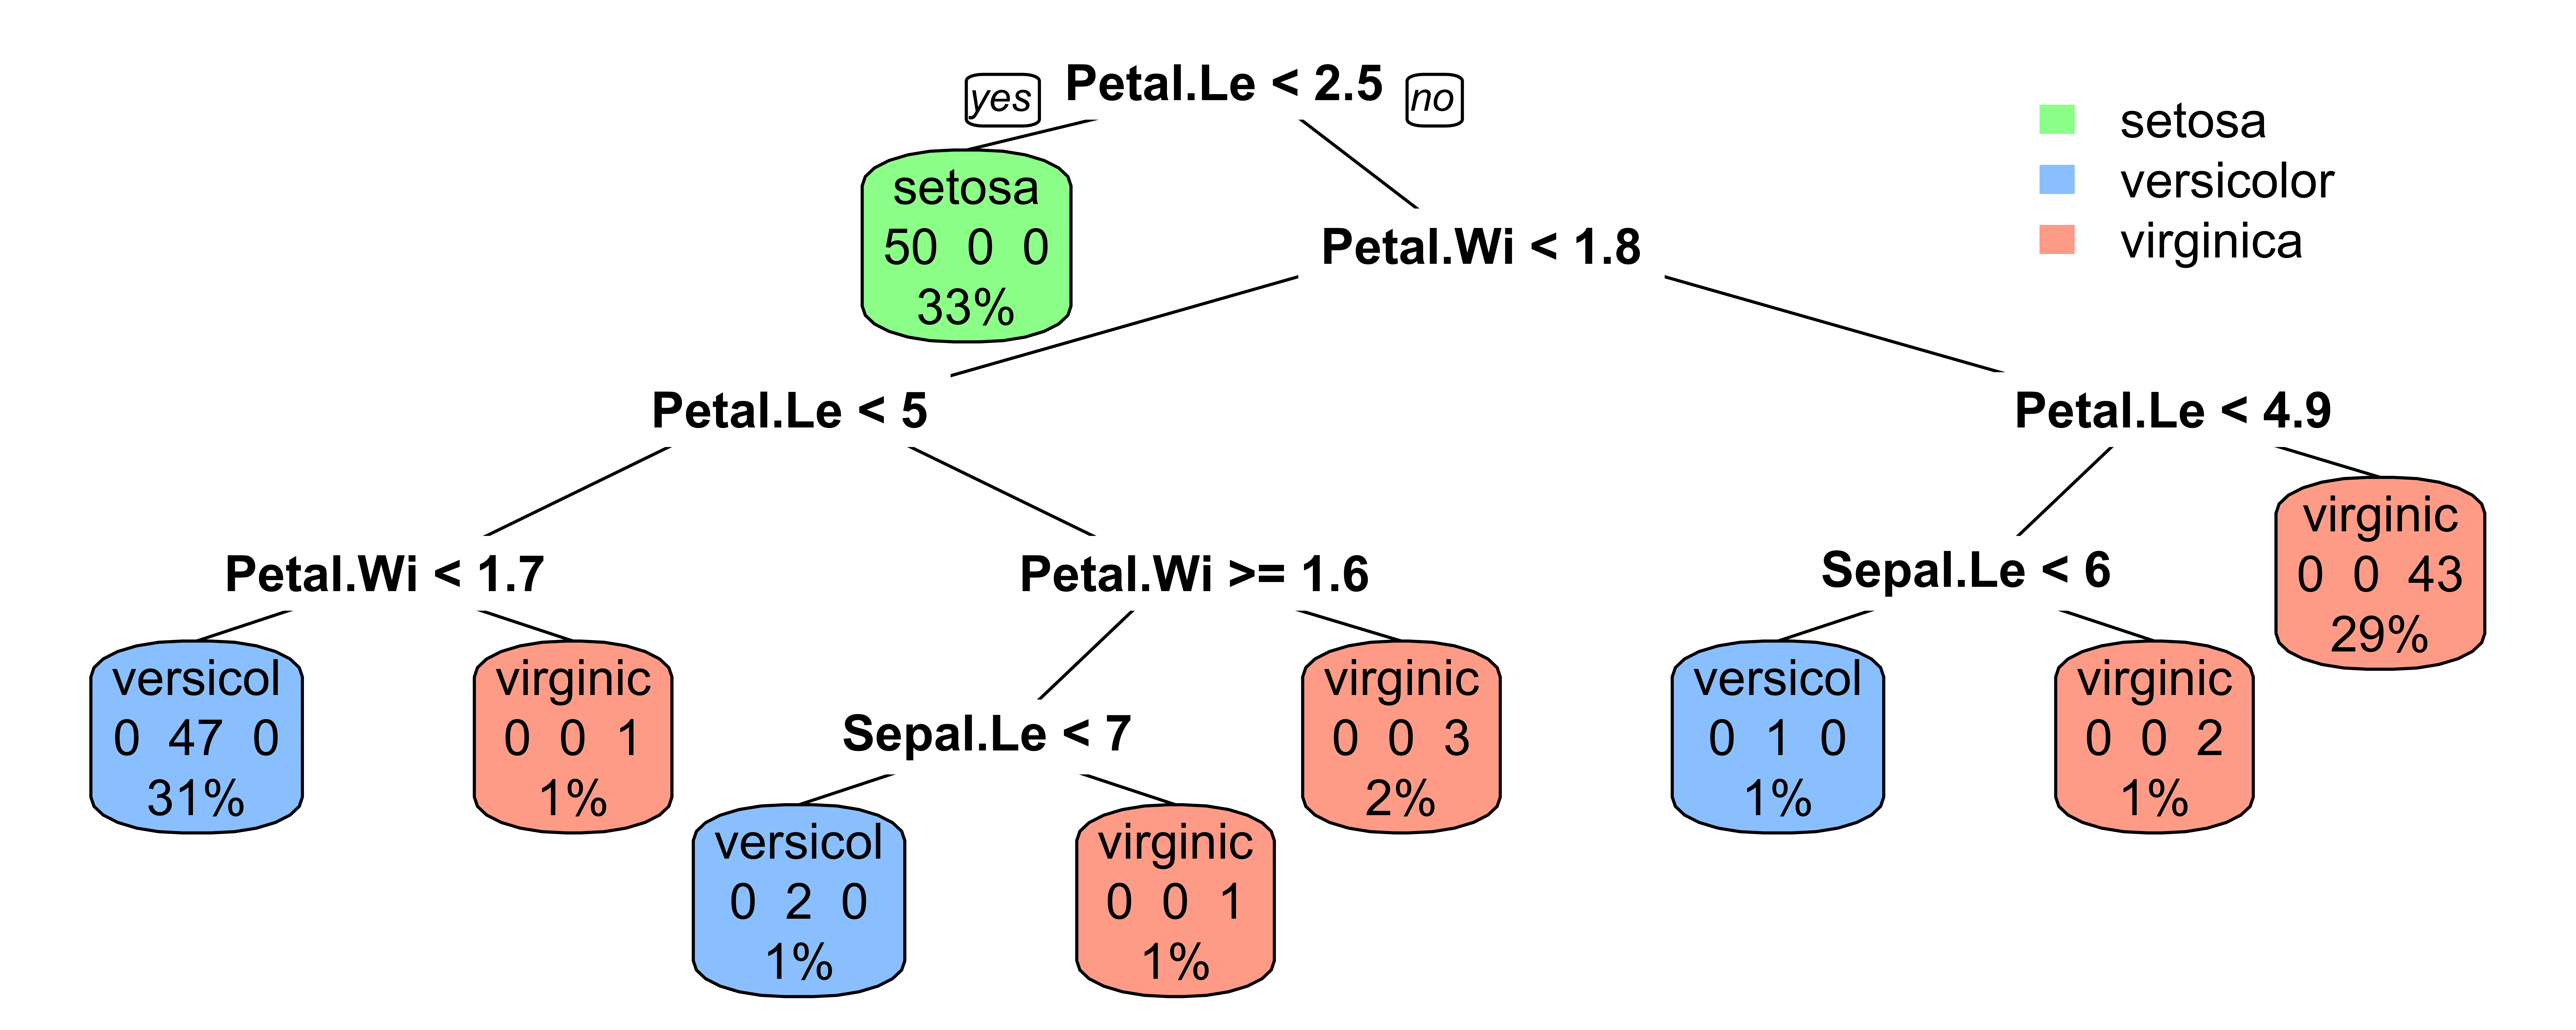
\includegraphics[height=3.5cm]{graphics/plot-rpart.png}
	\vskip 0.1cm 
	{\color{white}AA}
	\includegraphics[height=3.5cm]{graphics/scatter-petalLength-vs-petalWidth-boundaries.png}
	%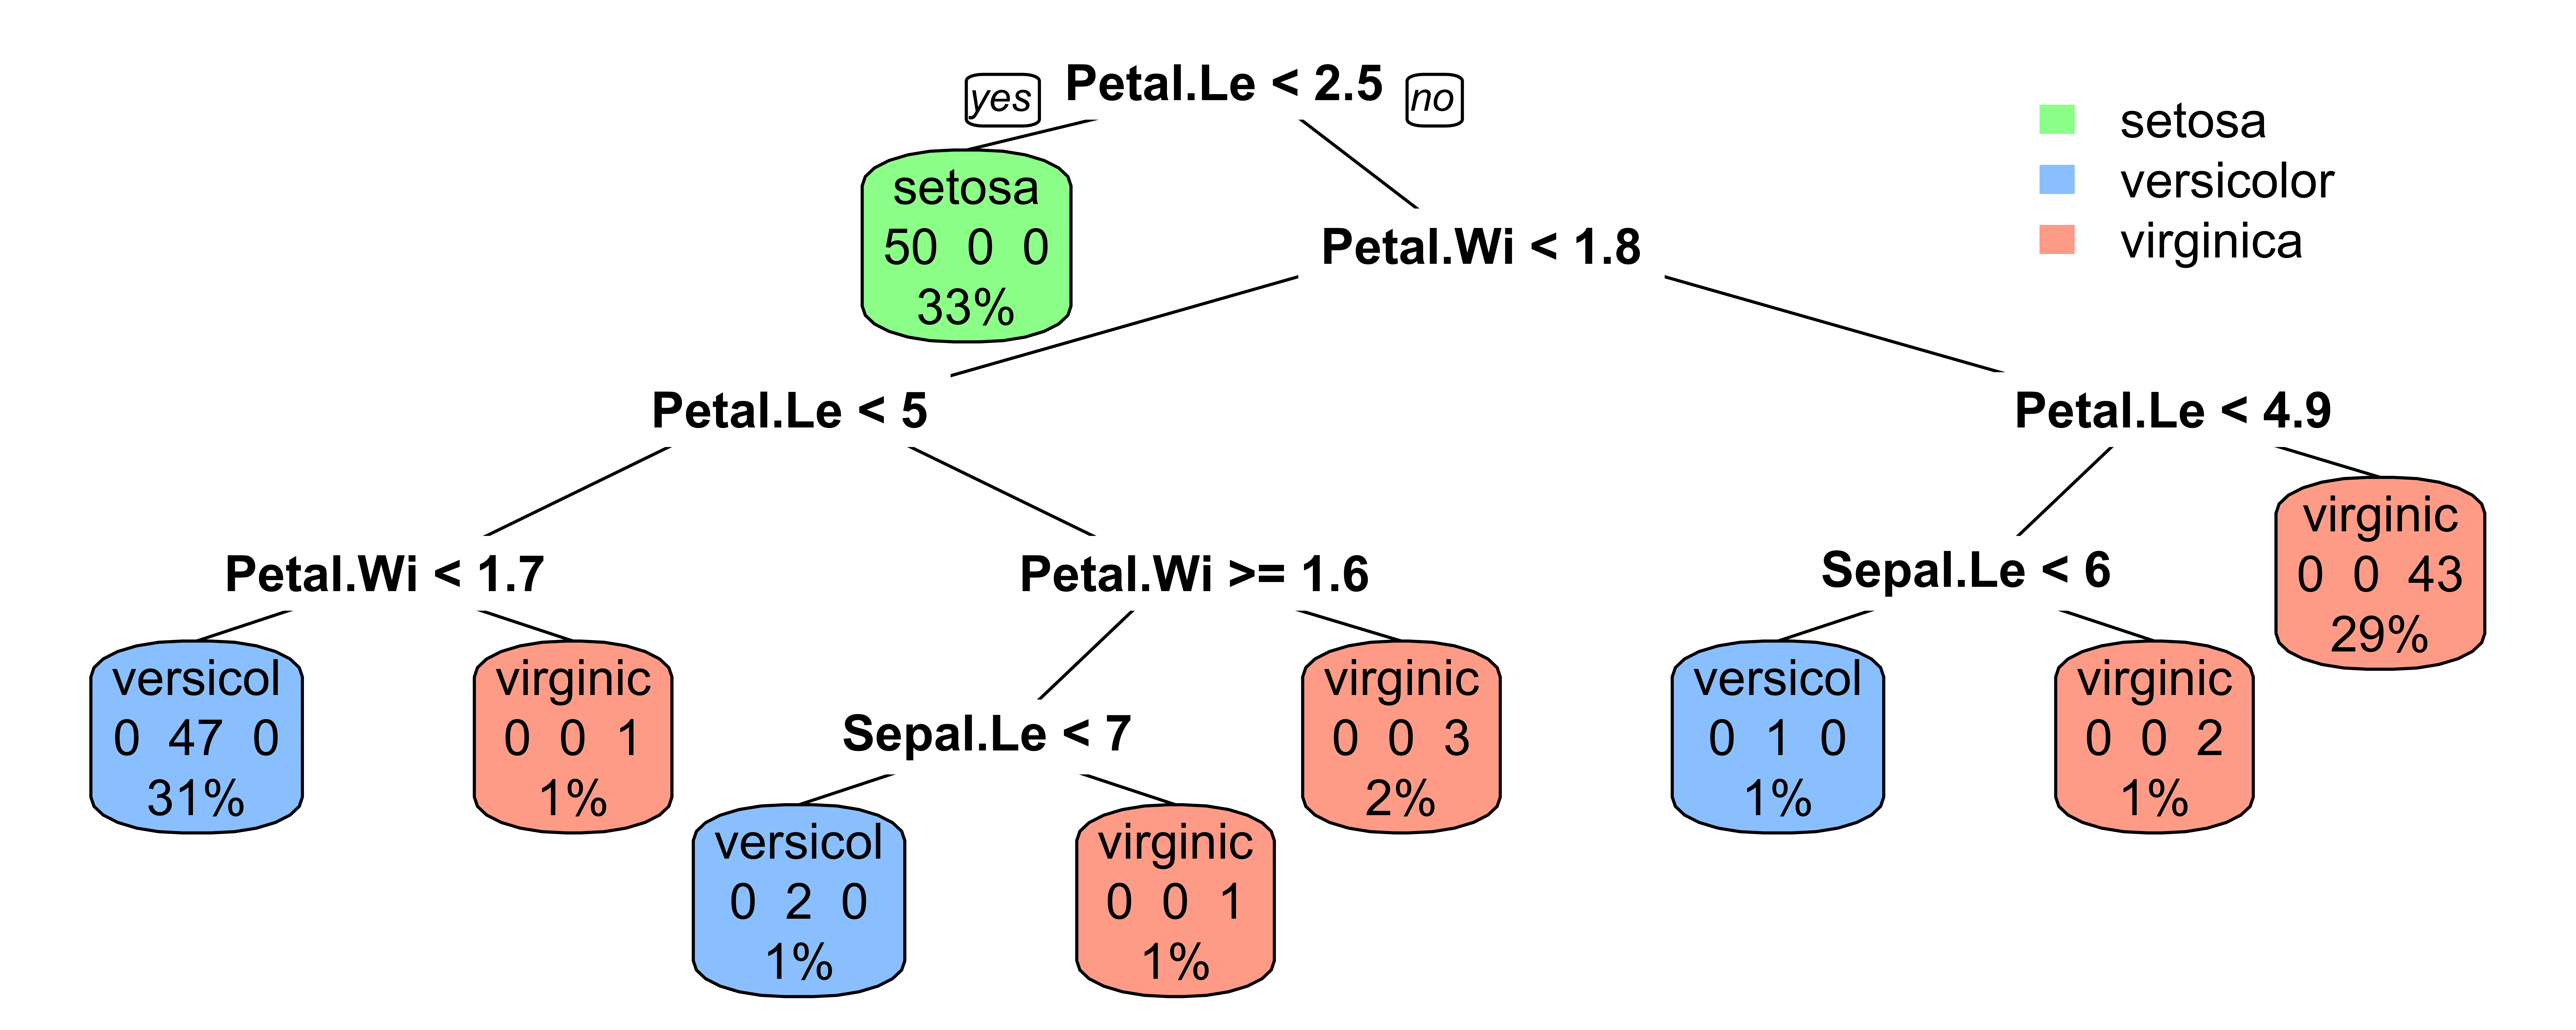
\includegraphics[width=4.5cm,height=6.25cm]{graphics/plot-rpart.png}
	%\includegraphics[width=4.5cm]{graphics/scatter-petalLength-vs-petalWidth-boundaries.png}
	\end{minipage}
	\end{flushright}

\columnbreak

	\begin{flushleft}
	\begin{minipage}{5.75cm}
	%\vskip -0.8cm
	%{\tiny
	%\begin{itemize}
	%\item
	%	\pause
	%	Goal: to find the impurity-minimizing tree.
	%\item
	%	\pause
	%	Hypothesis class is ``essentially'' finite (given data),
	%	but usually too enormous;
	%	\pause
	%	exhaustive search won't work.
	%\end{itemize}}
	\vskip -0.1cm
	\scriptsize
	\pause
	\textbf{\normalsize CART algorithm} (tree-growing step)
	\begin{itemize}
	\item
		\pause
		At each iteration, binary-partition \textbf{\color{red}each} leaf to get the next tree.
	\item
		\pause
		For each leaf, thus need to choose:
		\vskip -0.2cm
		\begin{itemize}
		\setlength{\itemindent}{-0.2in}
		\item
			\pause
			\vskip -0.1cm {\scriptsize``best'' predictor variable to partition by}
		\item
			\pause
			\vskip -0.1cm {\scriptsize``best'' threshold}
		\end{itemize}
	\item
		\pause
		Jensen's inequality \,$\Longrightarrow$\,
		{\color{red}Tree impurity always decreases after partitioning a leaf.}
	\item
		\pause
		For each leaf, choose the (variable,{\color{white}.}threshold)-combo
		that maximizes impurity decrease.
	\item
		\pause
		For each leaf, continue until termination criteria are met.
	%\item
	%	\pause
	%	Computational complexity = $O\!\left(p\,n \log n\right)$
	\end{itemize}
	\end{minipage}
	\end{flushleft}

\end{multicols}

\end{frame}
\normalsize

%%%%%%%%%%

\begin{frame}{\vskip -0.2cm \large The Breiman-Friedman-Olshen-Stone CART Algorithm}

\Large
\textbf{CART Algorithm} (tree-pruning step)

\vskip 0.1cm
\scriptsize
\begin{itemize}
\pause
\item
	For details see:
	\vskip -0.2cm
	{\tiny\begin{itemize}
	\item
		{\tiny Breiman-Friedman-Olshen-Stone, (1984),
		\textit{Classification and Regression Trees}, Taylor \& Francis}
	\item
		\vskip -0.1cm
		{\tiny Ripley, (1996),
		\textit{Pattern Recognition and Neural Networks}, Cambridge University Press}
	\end{itemize}}
\pause
\item
	The tree-growing step tends to produce overfit trees.
\pause
\item
	Grow-then-prune works better than grow-only with strong termination criteria:
	poor-at-first-glance splits may lead to very good splits further down the tree.
\pause
\item
	Once the full tree \,$T_{0}$\, has been grown, use \textbf{cost complexity criterion}
	\vskip -0.1cm
	\begin{equation*}
	C_{{\color{red}\alpha}}(T) \;\; = \;\;
		\#\textnormal{\scriptsize$\left(\!\begin{array}{c}
			\textnormal{misclassified}
			\\
			\textnormal{observations}
		\end{array}\!\right)$}
		\; + \;
		{\color{lightRed}\alpha} \cdot
		\#\textnormal{\scriptsize$\left(\!\begin{array}{c}
			\textnormal{leafs}
			\\
			\textnormal{of $T$}
		\end{array}\!\right)$}
	\end{equation*}
	\vskip -0.1cm
	to assess a given sub-tree $T \subset T_{0}$.
\item
	Fact:
	{\color{red}For each $\alpha \geq 0$,
	\,$T_{\alpha}$ $=$
	$\underset{T \subset T_{0}}{\textnormal{argmin}}\!\left\{\,\overset{{\color{white}.}}{C}_{\alpha}(T)\,\right\}$\,
	exists, is unique, and is computable.}
\item
	To choose optimal $\alpha$, use $5$- or $10$-fold cross-validation:
	Minimize cross-validation misclassification error of $T_{\alpha}$.
\end{itemize}

\end{frame}
\normalsize

%%%%%%%%%%


%%%%%%%%%%

\begin{frame}{\vskip -0.2cm \Large Forces et faiblesses des arbres de classification}

\vskip 0.3cm

\scriptsize
\pause
{\large Forces}
\vskip 0.05cm
\begin{itemize}
\pause
\item
	{\normalsize Facile \`a interpr\'eter}
	\vskip 0.1cm
	prise de d\'ecisions (presque) visuellement claire 

\vskip 0.25cm
\pause
\item
	{\normalsize faible biais / petite erreur d'entra\^{i}nement}
	\vskip 0.1cm
	gr\^{a}ce \`{a} la complexit\'{e} de sa classe d'hypoth\`eses
\end{itemize}

\vskip 0.3cm
\pause
{\large Faiblesses}
\vskip 0.05cm
\begin{itemize}
\pause
\item
	{\normalsize Variance \'elev\'ee / importante erreur de g\'en\'eralisation / avoir tendance \`a sur-entra\^iner}
	\vskip 0.1cm
	\`{a} cause de la complexit\'{e} de sa classe d'hypoth\`eses

\vskip 0.3cm
\pause
\item
	{\normalsize Fortes hypoth\`{e}ses g\'eometriques implicites artificielles :}
	\vskip 0.1cm
	Les arbres entra\^{i}n\'es correspondent aux fonctions constantes par morceaux
	sur les hyper-rectangles avec fronti\`eres
	parall\`{e}les aux hyperplans de coordonn\'ees dans l'espace des variables pr\'edictives
	
\vskip 0.3cm
\pause
\item
	{\normalsize Instabilit\'{e}}
	\vskip 0.1cm
	Les arbres entra\^{i}n\'es sensibles \`a de failbles perturbations des donn\'{e}es
\end{itemize}

\end{frame}
\normalsize

%%%%%%%%%%


%%%%%%%%%%

\begin{frame}{\vskip -0.4cm \large Implicit geometric assumptions of classification trees}

\begin{center}
\vskip -0.1cm
\includegraphics[height=3.5cm,width=3.5cm]{graphics/plot-horizontal-scatter.png}
\quad\quad
\includegraphics[height=3.5cm,width=2.5cm]{graphics/plot-horizontal-tree.png}
\end{center}

\begin{center}
\includegraphics[height=3.5cm,width=3.5cm]{graphics/plot-diagonal-scatter.png}
\quad\quad
\includegraphics[height=3.5cm,width=2.5cm]{graphics/plot-diagonal-tree.png}
\end{center}

\end{frame}
\normalsize

%%%%%%%%%%


%
%%%%%%%%%%%%%%%%%%%%%%%%%%%%%%%%%%%%%%%%%%%%%%%%%%
\begin{frame}{}

\begin{center}
\vskip 2.5cm
\resizebox{\linewidth}{!}{\itshape Merci !!}
\end{center}

\begin{center}
\vskip 0.5cm
{\Large Kenneth Chu}
\vskip 0.1cm
\texttt{kenneth.chu@canada.ca}
\vskip 0.1cm
{\small Enqu\^{e}tes sp\'{e}ciales, transport, technologie et assurance de la qualit\'{e}, DMEE
\vskip 0.0cm Special Surveys, Transportation, Technology and Quality Assurance, BSMD}
\end{center}

\end{frame}
\normalsize

%%%%%%%%%%%%%%%%%%%%%%%%%%%%%%%%%%%%%%%%%%%%%%%%%%


%%%%%%%%%%%%%%%%%%%%%%%%%%%%%%%%%%%%%%%%%%%%%%%%%%%

\begin{frame}{\vskip -0.1cm \huge Personnes-ressources}

\large

\begin{center}
\begin{multicols}{2}
	\begin{minipage}{4.5cm}
	\vskip -2.6cm
	\begin{center}
	Pour plus d'information,
	\vskip -0.01cm
	\noindent
	veuillez contacter :
	\end{center}
	\end{minipage}
\columnbreak
	\begin{minipage}{4.0cm}
	\vskip -2.5cm
	\begin{center}
	For more information,
	\vskip -0.01cm
	\noindent
	please contact\!:
	\end{center}
	\end{minipage}
\end{multicols}
\end{center}

\definecolor{darkBlue}{RGB}{40,80,204}

\begin{center}
\vskip 0.5cm
\textbf{\huge Kenneth\;\,Chu}
\vskip 0.15cm
%\texttt{\Large kenneth.chu@canada.ca}
\href{mailto:kenneth.chu@canada.ca}{\Large\color{darkBlue}\underline{\texttt{kenneth.chu@canada.ca}}}
\vskip 0.24cm
\texttt{\Large 613-852-7361}
\end{center}
%
\end{frame}
%\normalsize

%%%%%%%%%%%%%%%%%%%%%%%%%%%%%%%%%%%%%%%%%%%%%%%%%%%
%\begin{frame}{}
%
%\begin{center}
%\vskip 2.5cm
%\resizebox{\linewidth}{!}{\itshape Merci !!}
%\end{center}
%
%\begin{center}
%\vskip 0.5cm
%{\Large Kenneth Chu}
%\vskip 0.1cm
%\texttt{kenneth.chu@canada.ca}
%\vskip 0.1cm
%{\small Enqu\^{e}tes sp\'{e}ciales, transport, technologie et assurance de la qualit\'{e}, DMEE
%\vskip 0.0cm Special Surveys, Transportation, Technology and Quality Assurance, BSMD}
%\end{center}
%
%\end{frame}
%\normalsize
%
%%%%%%%%%%%%%%%%%%%%%%%%%%%%%%%%%%%%%%%%%%%%%%%%%%%


%%%%% ~~~~~~~~~~~~~~~~~~~~ %%%%%
%\appendix
%
%%%%%%%%%%

\begin{frame}{\vskip -0.2cm \normalsize Discussion}

\vskip -0.2cm
\begin{itemize}\scriptsize
\item
	Possible ML techniques to showcase in demo pipelines:
	\begin{itemize}\tiny
	\item
		Classification: support vector machines, decision trees, random forests, nearest neighbour, neural networks
	\item
		Regression: support vector machines, random forests, regularized regression
	\item
		Unsupervised learning: clustering, PCA, dimension reduction, etc.
	\end{itemize}

\item
	Contents of demo pipelines:
	\begin{itemize}\tiny
	\item
		Master program (philosophy: one ``click'' makes all)
	\item
		README file: how to run the master program, refer user to blog post on Confluence page for associated blog.
	\item
		Documentation in code
	\item
		Optional: PDF version of associated blog post to explain the ML technique of the demo pipeline
	\end{itemize}

\item
	Outreach activities
	\begin{itemize}\tiny
	\item
		Publish blog posts on Confluence page about demo pipelines.
	\item
		Share demo pipelines as ZIP files through the associated blog posts.
	\item
		Give branch-level seminars -- probably a series of two back-to-back seminars
	\item
		Optional: use {\color{red}Jupyter} Notebook to give a live demo during seminars
	\item
		Optional: share demo pipelines through StatCan's (Team Foundation Service) Git repository on Network A.
	\end{itemize}

\item
	Proposed timeframe (subject to adjustment):
	\begin{itemize}\tiny
	\item
		Demo pipeline (choose ML technique, learn the technique, choose language, build demo pipeline):
	\item
		Blog posts:
	\item
		Seminars: \textbf{\color{red}Early February, 2018}
	\end{itemize}

\item
	Keywords:
	\begin{itemize}\tiny
	\item
		bagging, boosting, ensemble methods, deep learning
	\item
		sensitivity, specificity, precision, recall, confusion matrix, ROC Curve
	\end{itemize}

\end{itemize}

\end{frame}
\normalsize

%%%%%%%%%%


%%%%%%%%%%%%%%%%%%%%%%%%%%%%%%%%%%%%%%%%%%%%%%%%%%

\end{document}

%%%%%%%%%%%%%%%%%%%%%%%%%%%%%%%%%%%%%%%%%%%%%%%%%%
